\documentclass[10pt,twocolumn,letterpaper]{article}

\usepackage{cvpr}
\usepackage{microtype}
\usepackage{times}
\usepackage{epsfig}
\usepackage{graphicx}
\usepackage{amsmath}
\usepackage{amssymb}
\usepackage{caption}
\usepackage{subcaption}
\usepackage{booktabs}
\usepackage{floatrow}
\newfloatcommand{capbtabbox}{table}[][\FBwidth]
% Include other packages here, before hyperref.

% If you comment hyperref and then uncomment it, you should delete
% egpaper.aux before re-running latex.  (Or just hit 'q' on the first latex
% run, let it finish, and you should be clear).
\usepackage[pagebackref=true,breaklinks=true,letterpaper=true,colorlinks,linkcolor=blue,citecolor=blue,bookmarks=false]{hyperref}

\newcommand{\JT}[1]{\textcolor{blue}{JT: #1}}
\newcommand{\HP}[1]{\textcolor{red}{HP: #1}}
\newcommand{\DFH}[1]{\textcolor{red}{DH: #1}}

% \cvprfinalcopy % *** Uncomment this line for the final submission

\def\cvprPaperID{0947} % *** Enter the CVPR Paper ID here
\def\httilde{\mbox{\tt\raisebox{-.5ex}{\symbol{126}}}}

% Pages are numbered in submission mode, and unnumbered in camera-ready
\ifcvprfinal\pagestyle{empty}\fi
\begin{document}

%%%%%%%%% TITLE
\title{Guided Proofreading of Automatic Segmentations for Connectomics\\~\\\textit{Supplemental Material}}

\author{Daniel Haehn\\
Institution1\\
Institution1 address\\
{\tt\small haehn@seas.harvard.edu}
% For a paper whose authors are all at the same institution,
% omit the following lines up until the closing ``}''.
% Additional authors and addresses can be added with ``\and'',
% just like the second author.
% To save space, use either the email address or home page, not both
\and
Second Author\\
Institution2\\
First line of institution2 address\\
{\tt\small secondauthor@i2.org}
}

\maketitle
%\thispagestyle{empty}

%%%%%%%%% ABSTRACT

%%%%%%%%% BODY TEXT

\section{Classifier}

\subsection{Architecture}
We explored different architectures for the convolutional neural network (CNN) for split error detection. We compare traditional CNN architectures versus residual networks~\cite{resnet} (Tab.~\ref{tab:architecture}). The traditional architecture with dropout regularization generalized better than residual networks on unseen testing data.

\begin{table}[t]
\caption{Traditional CNN Architecture versus Residual Network Architecture \cite{resnet}. All configurations are compared using the same parameters. Our final choice (indicated by *) trains relatively fast and performs better.}%While the training of our classifier is more expensive, testing accuracy is superior. }

\small{
\begin{tabular}{@{}ll|l@{}}
	\toprule
     ~ & \textbf{Traditional Network} & \textbf{Residual Network}  \\ \midrule	
\begin{tabular}{@{}r|@{}}
Conv. Layers \\
Dropout Reg. \\
Cost [m] \\
Test. Acc. \\
Prec./Recall \\
F1 Score\\
~
\end{tabular} & 
\begin{tabular}{@{}c|c@{}}
 2 & 4 \\
 y & y \\
 27.5 & 383 \\
 0.925 & 0.94 \\
 0.93/0.93 &
 0.94/0.94 \\
 0.93 & 0.94 \\
 ~&*
\end{tabular}
& 
\begin{tabular}{@{}c|c@{}}
 5 & 13 \\
 y & n \\
5080 & 1094 \\
 0.93 & 0.90 \\
 0.7/0.53 &
 0.74/0.66 \\
 0.39 & 0.64\\
 ~&~

\end{tabular}

\end{tabular}
\hspace{2mm}
\hrule
}
\label{tab:architecture}
\end{table}




\subsection{Training Parameters}

We performed a limited brute force parameter search to tune the split error classifier (Tab.~\ref{tab:parametersearch}). This resulted in 3240 different CNN configurations which were evaluated on 10\% of our training data. Learning rate and momentum ranges are defined linearly across 2000 epochs.

\begin{table}[t]
\caption{Brute force parameter search for the split error classifier. The final parameters are highlighted.}%While the training of our classifier is more expensive, testing accuracy is superior. }

\small{
\begin{tabular}{@{}ll}
	\toprule
     \textbf{Parameter} & \textbf{Search Space}  \\ \midrule	
\begin{tabular}{@{}l@{}}
Filter size: \\
No. Filters 1: \\
No. Filters 2-4: \\
Dense units:\\
Learning rate: \\
Momentum: \\
Mini-Batchsize: 
\end{tabular} & 
\begin{tabular}{@{}l@{}}
\textbf{3x3}, 5x5, 9x9, 13x13\\
32, 48, \textbf{64} \\
32, \textbf{48}, 64 \\
256, \textbf{512} \\
0.00001, 0.0001, 0.001, 0.01, \textbf{0.03-0.00001} \\
0.9, 0.95, \textbf{0.9-0.999} \\
10, 100, \textbf{128}
\end{tabular}

\end{tabular}
\hspace{2mm}
\hrule
}
\label{tab:parametersearch}
\end{table}

\subsection{Automatic Method Threshold $p_t$}
For automatic selection, we observed a threshold $p_t=0.95$ as stable when evaluating on previously unseen testing data (Mouse S1 AC3 Open Connectome Project dataset). This means that automatic selection stops once all borders with $p_t\geq0.95$ were proofread. Figure~\ref{fig:cylboxplot} shows split error classification on three randomly selected subvolumes ($700\times700\times2$ voxels) of AC3. In all cases, the threshold $p_t=0.95$ reduces VI.

\begin{figure}[t]
\centering
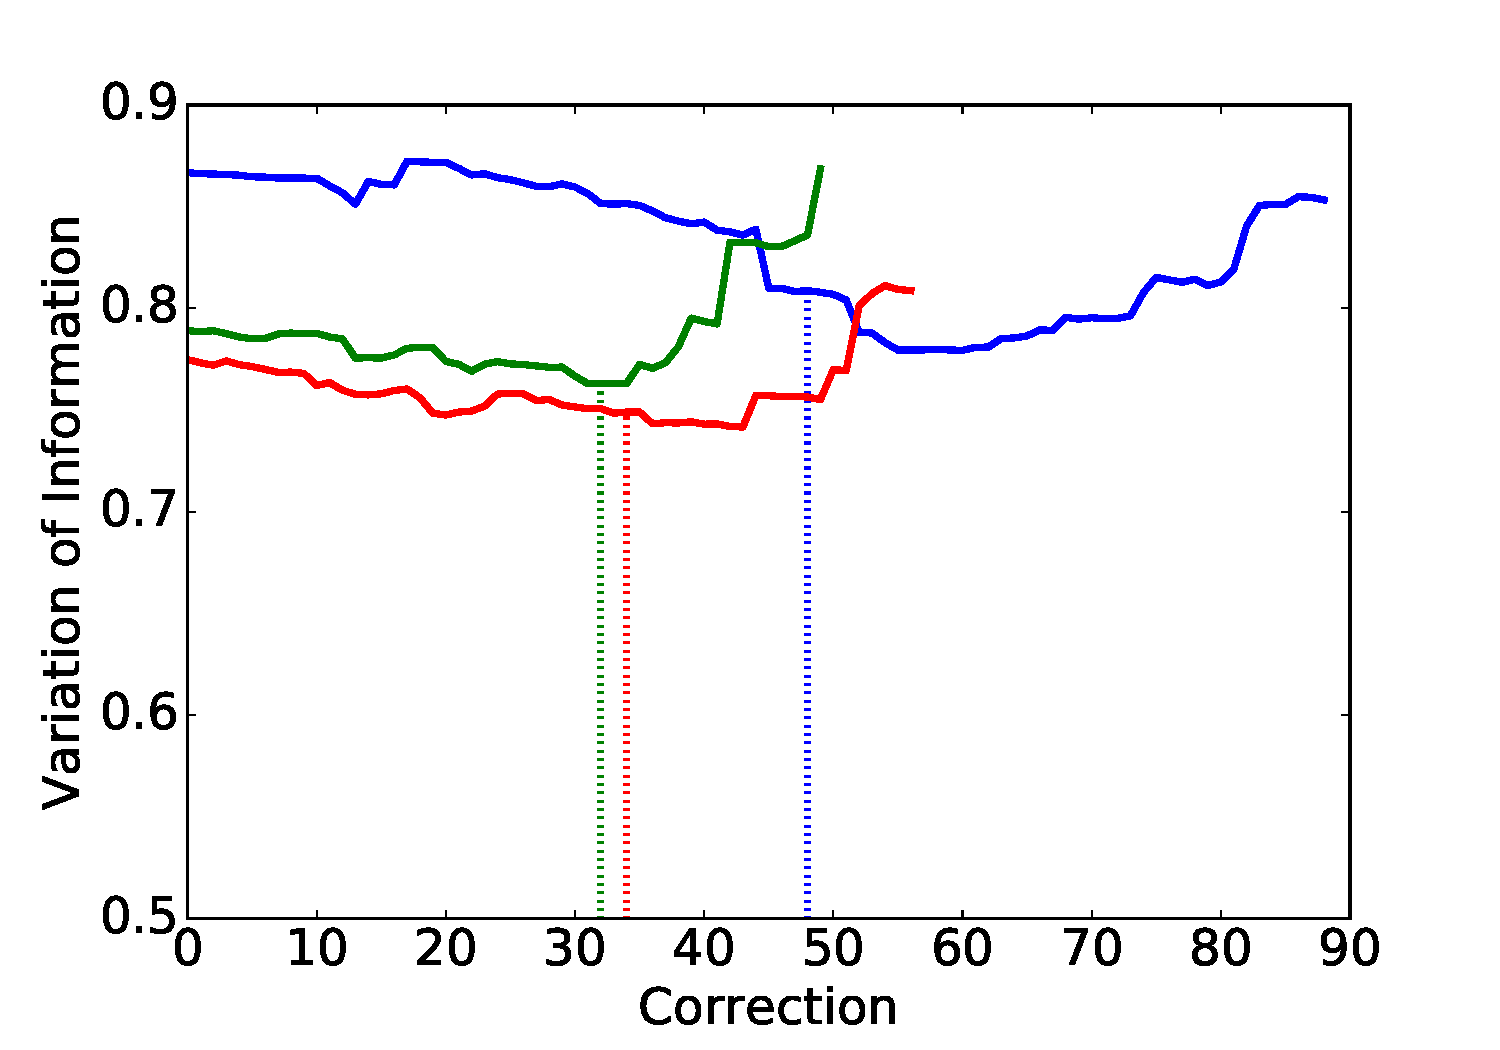
\includegraphics[width=\linewidth]{gfx/ptplot.pdf}
\caption{Observations of probability thresholds $p_t$ during automatic selection on three different subvolumes of previously unseen testing data. The dashed lines show when $p_t=0.95$ is reached.}
\label{fig:cylboxplot}
\end{figure}

\subsection{Limitations}
Guided proofreading works on 2D image sections. This enables error correction without a computationally expensive alignment process. However, the output requires an additional (block-)merging step prior to 3D analysis. Several software packages exist for this purpose.

As described in section~\ref{sec:addexp}, the guided proofreading classifier has to be retrained if used on a different species than mouse. Parameters do not need to be changed.


\section{L. Cylinder Results}

\begin{figure}[t]
\centering
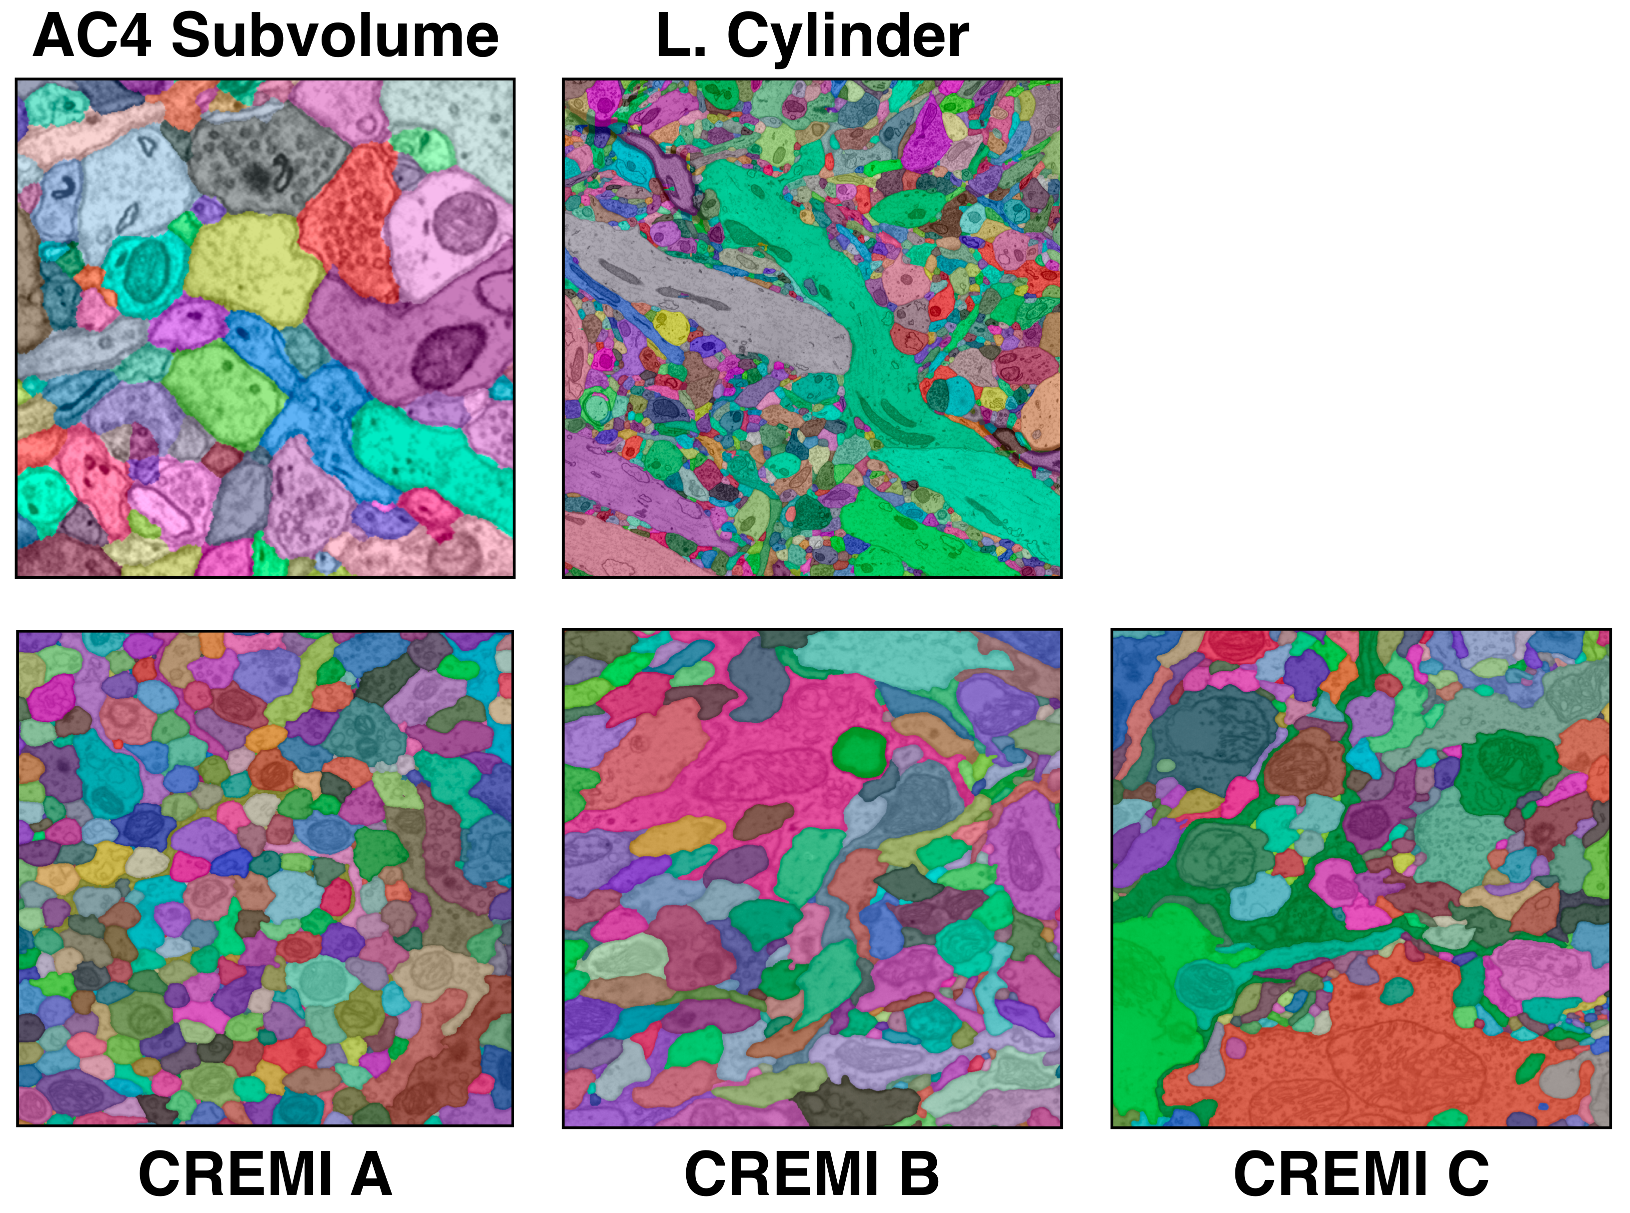
\includegraphics[width=\linewidth]{gfx/datasets.png}
\caption{The five different datasets we use for evaluation. The top row shows the first slice of the AC4 and L.~Cylinder mouse brain datasets as reported in the paper. The bottom row shows the first slice of the CREMI A/B/C fruit fly datasets which we used for additional experiments.}
\label{fig:datasets}
\end{figure}

We report experiments and results on the L.~Cylinder dataset in the paper. Figure~\ref{fig:cyltrails} and~\ref{fig:cylboxplot} visualize the reported results measured as variation of information (VI). We compare automatic selection with threshold and selection oracle using focused proofreading and guided proofreading.

\paragraph{Best possible VI.} The selection oracle using guided proofreading does not reach the best possible VI score. We calculate this score by intersecting the initial segmentation and the ground truth. In theory, the classifier should be able to reach this lower bound. However, due to the classification patch size, the membrane probability maps we used included a 30 pixel frame region. Guided proofreading ignores all segments within this frame region, and so cannot reach the best possible VI in some datasets.

\begin{figure}[t]
\centering
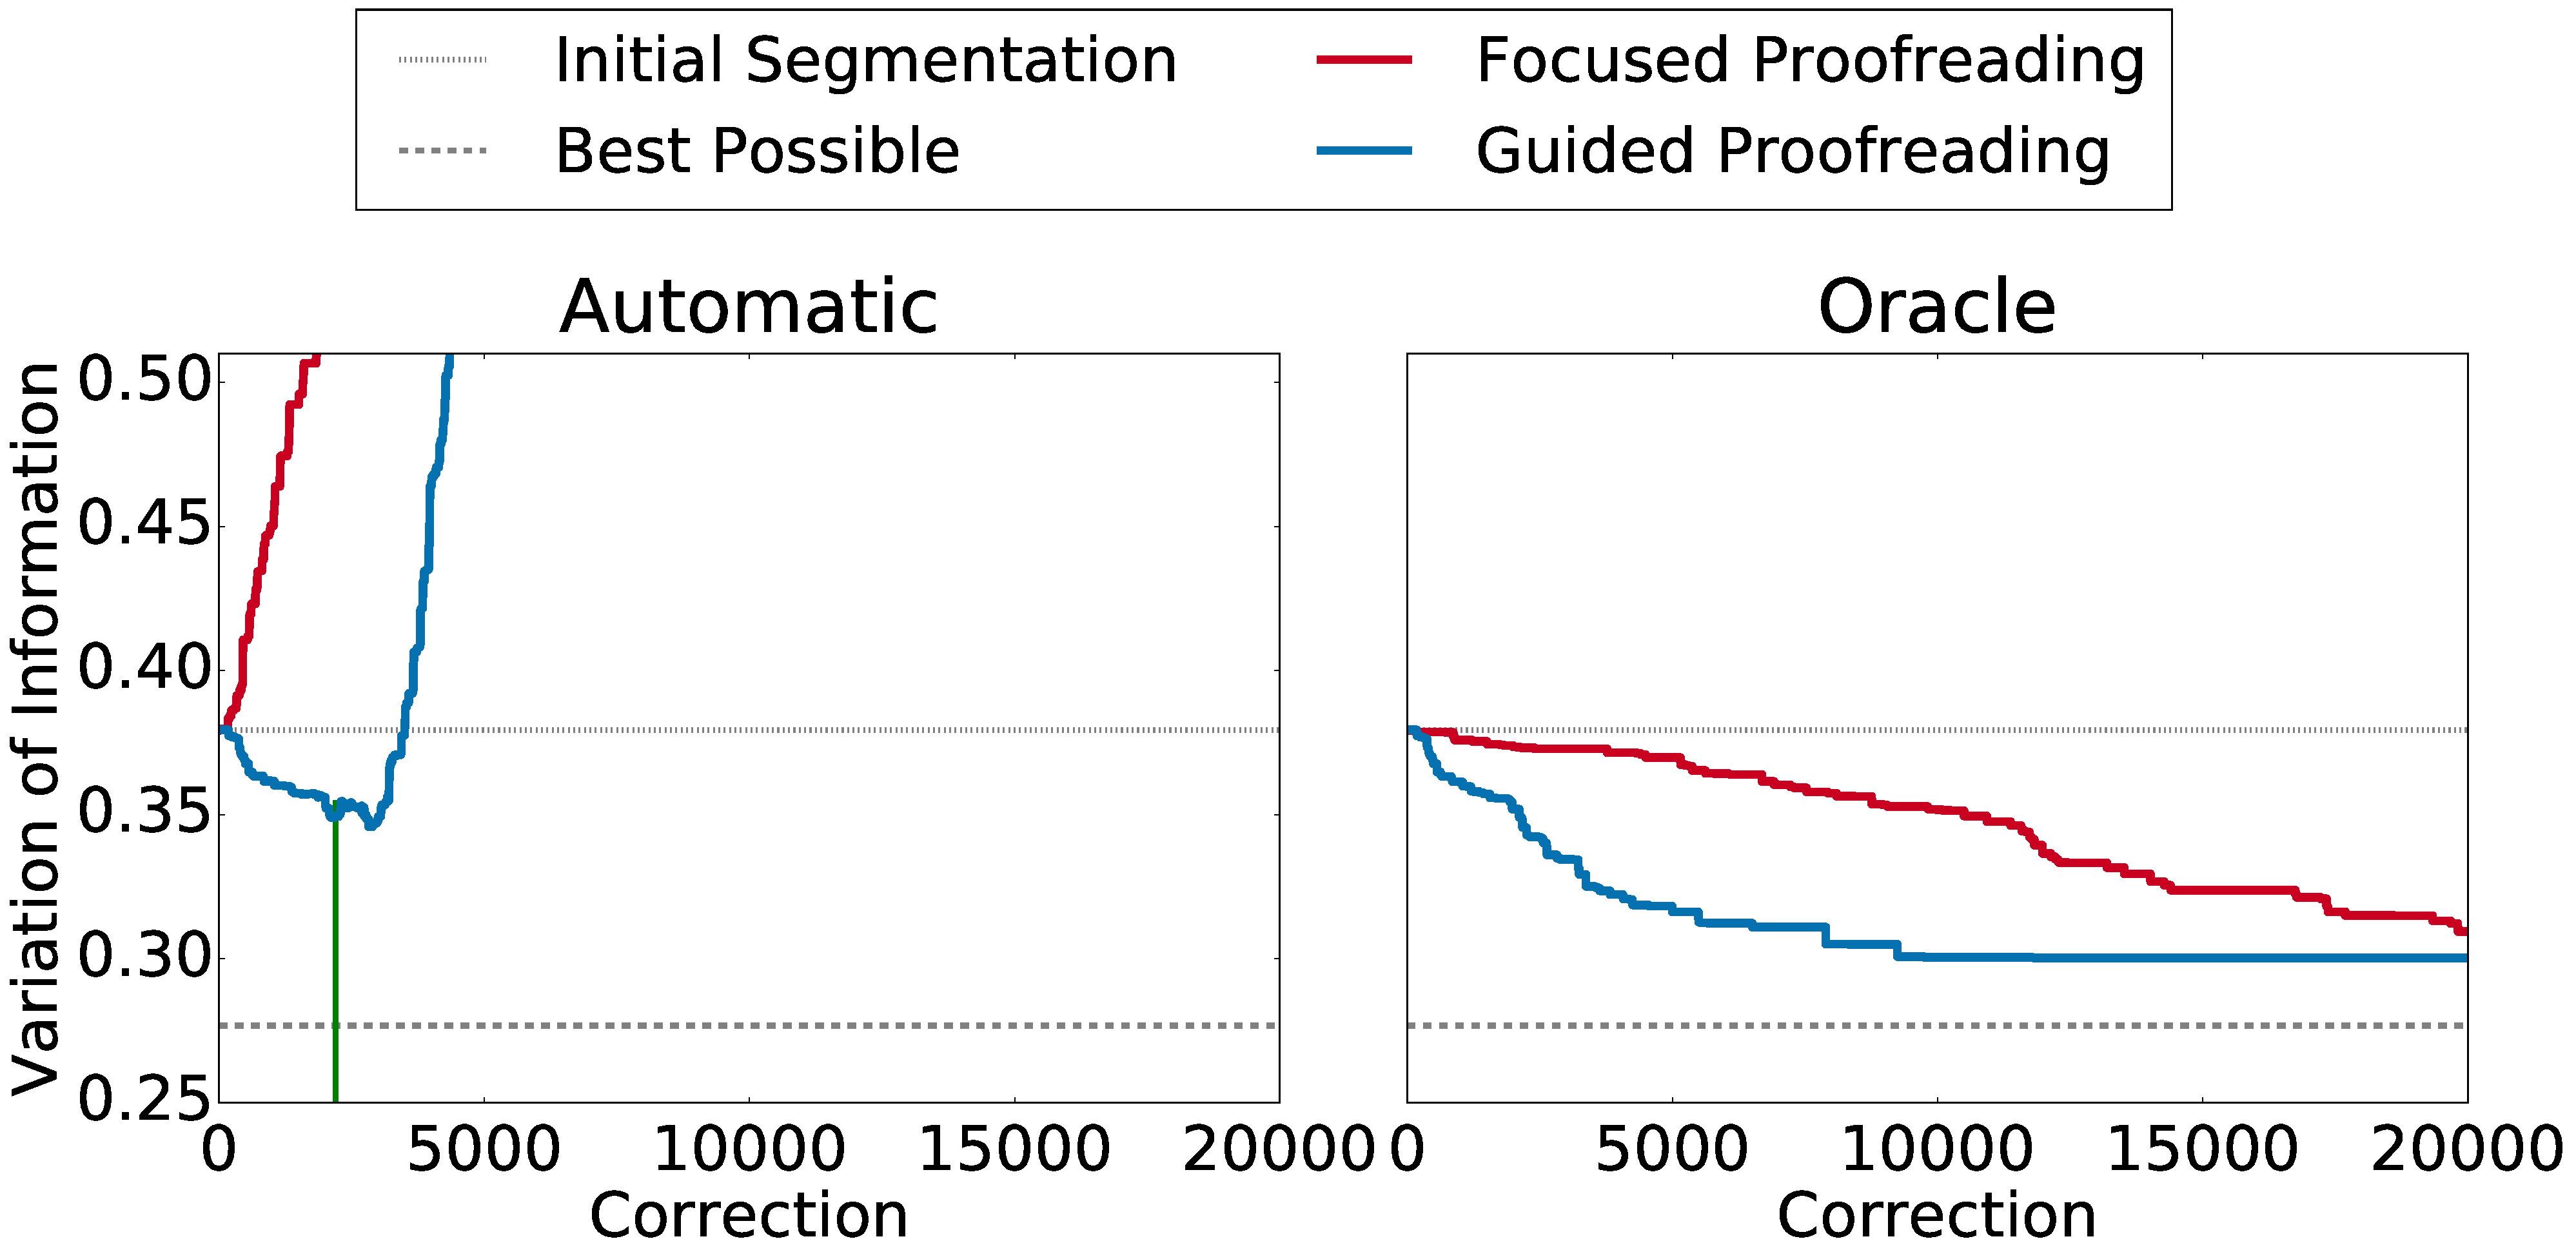
\includegraphics[width=\linewidth]{gfx/cyl_trails.pdf}
\caption{Performance comparison of Plaza's focused proofreading and our guided proofreading on the L.~Cylinder dataset as reported in the paper. All measurements are shown as median VI, the lower the better. We compare automatic selection with threshold ($p_t=0.95$, green line) and the selection oracle for accepting or rejecting corrections using each method. Guided proofreading yields better results faster with fewer corrections.}
\label{fig:cyltrails}
\end{figure}

\begin{figure}[t]
\centering
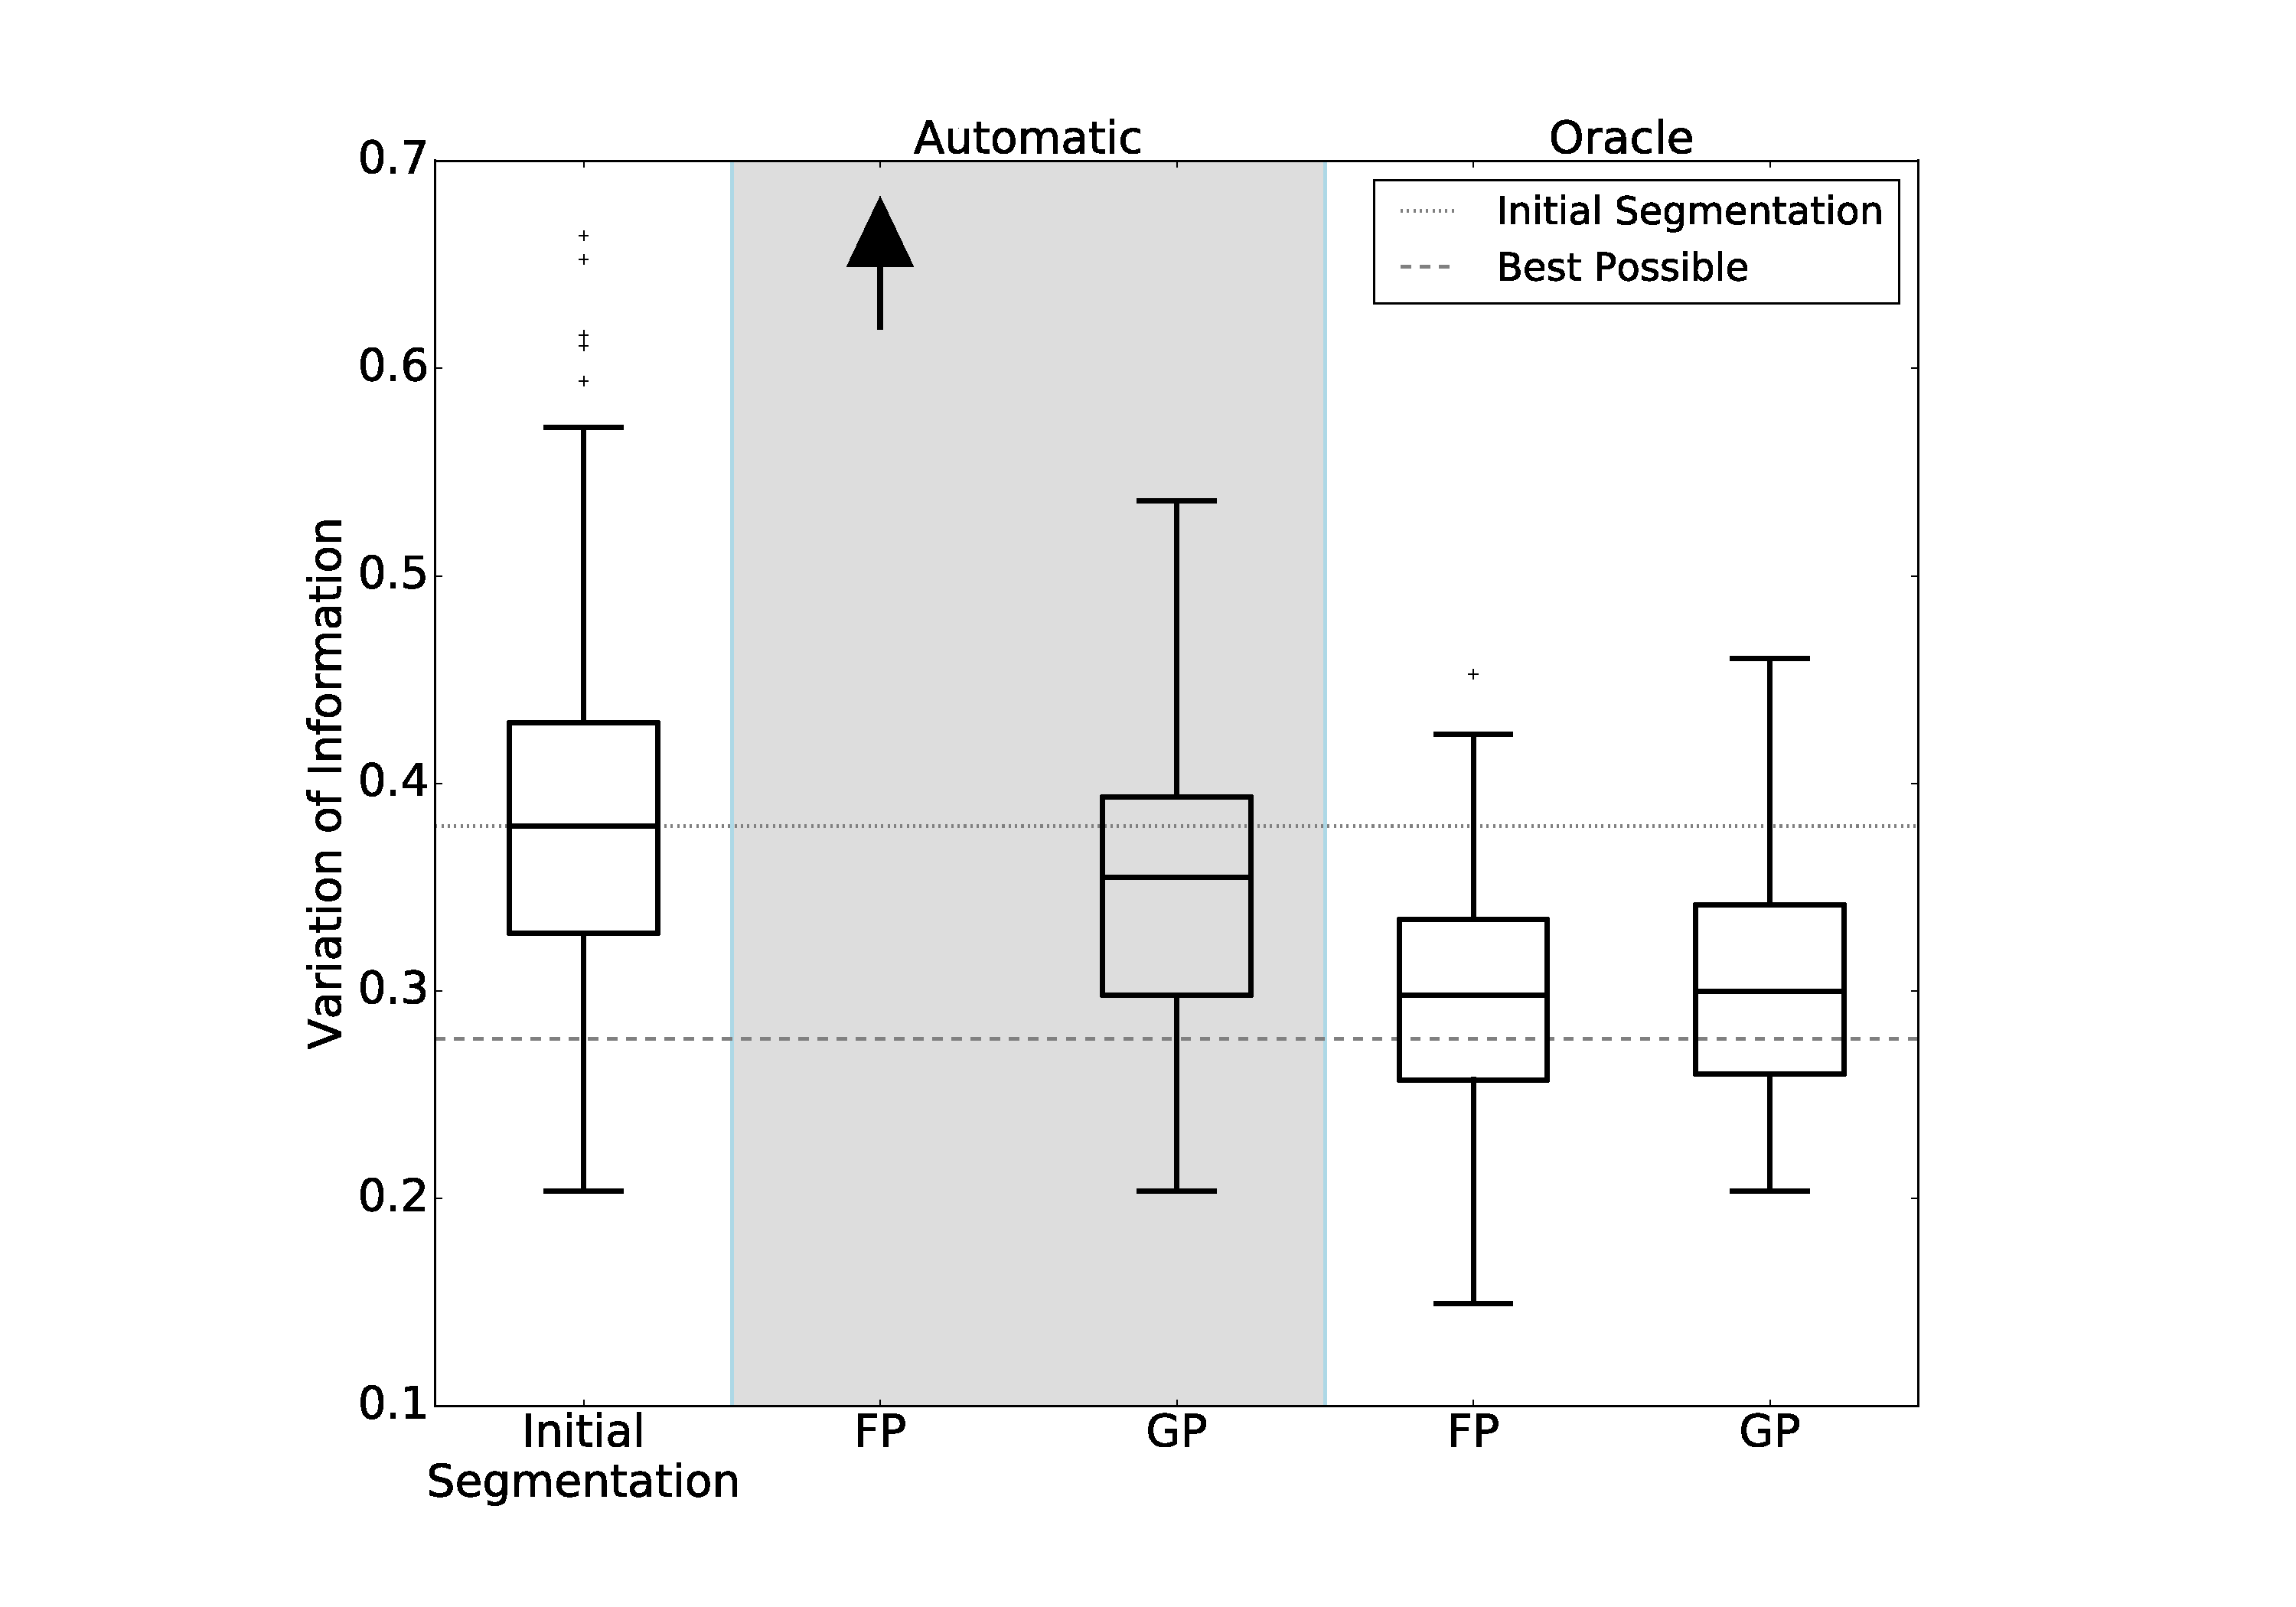
\includegraphics[width=\linewidth]{gfx/cylboxplot.pdf}
\caption{VI distributions of guided proofreading (GP) and focused proofreading (FP) output across slices of the L.~Cylinder dataset, with different error correction approaches. The variation resulting from performance of FP with automatic selection is $7.8\times$ higher than GP (\protect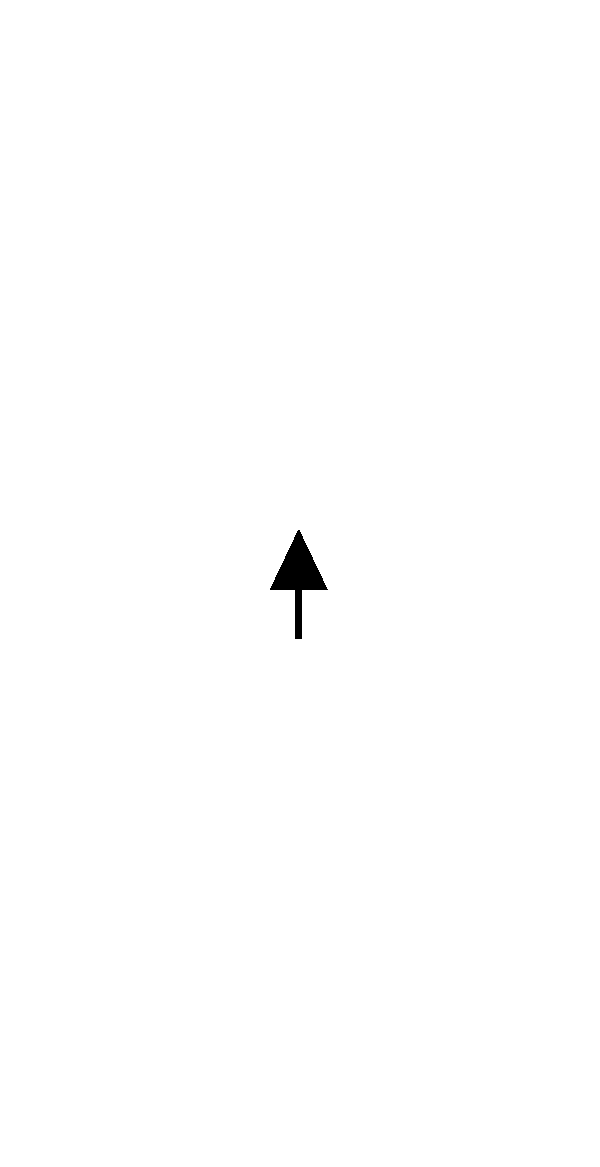
\includegraphics[width=0.2cm]{gfx/arrow.pdf}), with median VI of $2.75$ and $SD=0.789$.}
\label{fig:cylboxplot}
\end{figure}

\section{Confirmatory Data Analysis} 

We use a single factor between-subject design with the factor being the proofreading method (GP, FP, or Dojo). Our hypothesis is that VI reduction is significantly better with GP than with other tools. For this, we treat VI as a continuous variable and use analysis of variance (ANOVA~\cite{shaffer1995}) followed by parametric tests (Welch's t-test~\cite{welch}).

\paragraph{AC4 subvolume.} For novice performance, we observe a significant effect ($\alpha=0.05$) of which proofreading tool is used for the three conditions GP, FP, and Dojo [$F(2,27) = 6.446, p = 0.005$] when comparing the mean VI outcome. Post hoc comparisons (after Bonferroni correction) indicate that the mean VI for GP is significantly lower than for FP [$t_{27} = -2.7696, p = 0.0168$], and that the mean VI for GP is significantly lower than for Dojo [$t_{27} = -4.407, p < 0.001$]. This means that novices using GP perform significantly better than using FP and Dojo.
A similar trend is visible when comparing the expert performance between GP and FP as the change in mean VI of GP is significantly better ([$F(1,18) = 7.054, p = 0.016$] and [$t_{18} = -2.6559, p = 0.0216$]). For automatic selection with threshold, the difference in mean VI is very large and GP also performs significantly better ([$F(1,18) = 89.902, p < 0.001$] and [$t_{18} = 9.482, p < 0.001$]). The final VI scores of the selection oracle with GP and FP are very similar and the difference between them is not significant [$F(1,18) = 0.795, p = 0.384$]. However, the VI reduction rate of GP is much higher (Fig.~6, main paper, right).

\vspace{-4mm}

\paragraph{L. Cylinder.} The automatic selection with threshold yields similar results as on the AC4 dataset, and we observe a significant improvement when using GP instead of FP ([$F(1,98) = 26.676, p < 0.001$], post hoc comparison [$t_{98} = 5.1648, p < 0.001$]). The selection oracles of GP and FP result in very similar final VI scores and the difference is not significant [$F(1,98) = 0.071, p = 0.790$], but GP reaches minimum VI faster in $10,000$ corrections versus FP in $26,170$ corrections.
    
    
\section{Additional Experiments}
\label{sec:addexp}

\paragraph{CREMI A/B/C.} As part of the MICCAI 2016 challenge on circuit reconstruction from electron microscopy images (CREMI), six ssTEM datasets were made publicly available\footnote{\scriptsize{\url{http://www.cremi.org}}},  each $1250\times1250\times125$ voxels. Since only three datasets include manually-labeled `ground truth', we use these three volumes for our experiments. The volumes are part of an adult fruit fly (Drosophila melanogaster) brain. The resolution of all three datasets is $4\times4\times40~\text{nm}^3\text{/voxel}$.

\paragraph{Retraining.} Since the CREMI data is a different species, we simply retrain our split error classifier as well as focused proofreading by Plaza~\cite{focused_proofreading}. For this, we use the first 100 sections of each of the three CREMI datasets combined as training data. All parameters are unchanged and left as reported in the paper. 

\paragraph{Error correction.} In all three datasets merge error detection found over 300 merge errors. Unfortunately, merge error correction crashed because of a software error on our part. Therefore, we only evaluate split error detection and correction on subvolumes of CREMI A/B/C with the dimensions $1250\times1250\times5$ voxels. The subvolumes were cut from the last 25 sections of each of the three datasets and unseen during training. We compare focused proofreading and guided proofreading with automatic selection ($p_t=0.95$) and selection oracle.

\subsection{CREMI A}

\begin{figure}[t]
\centering
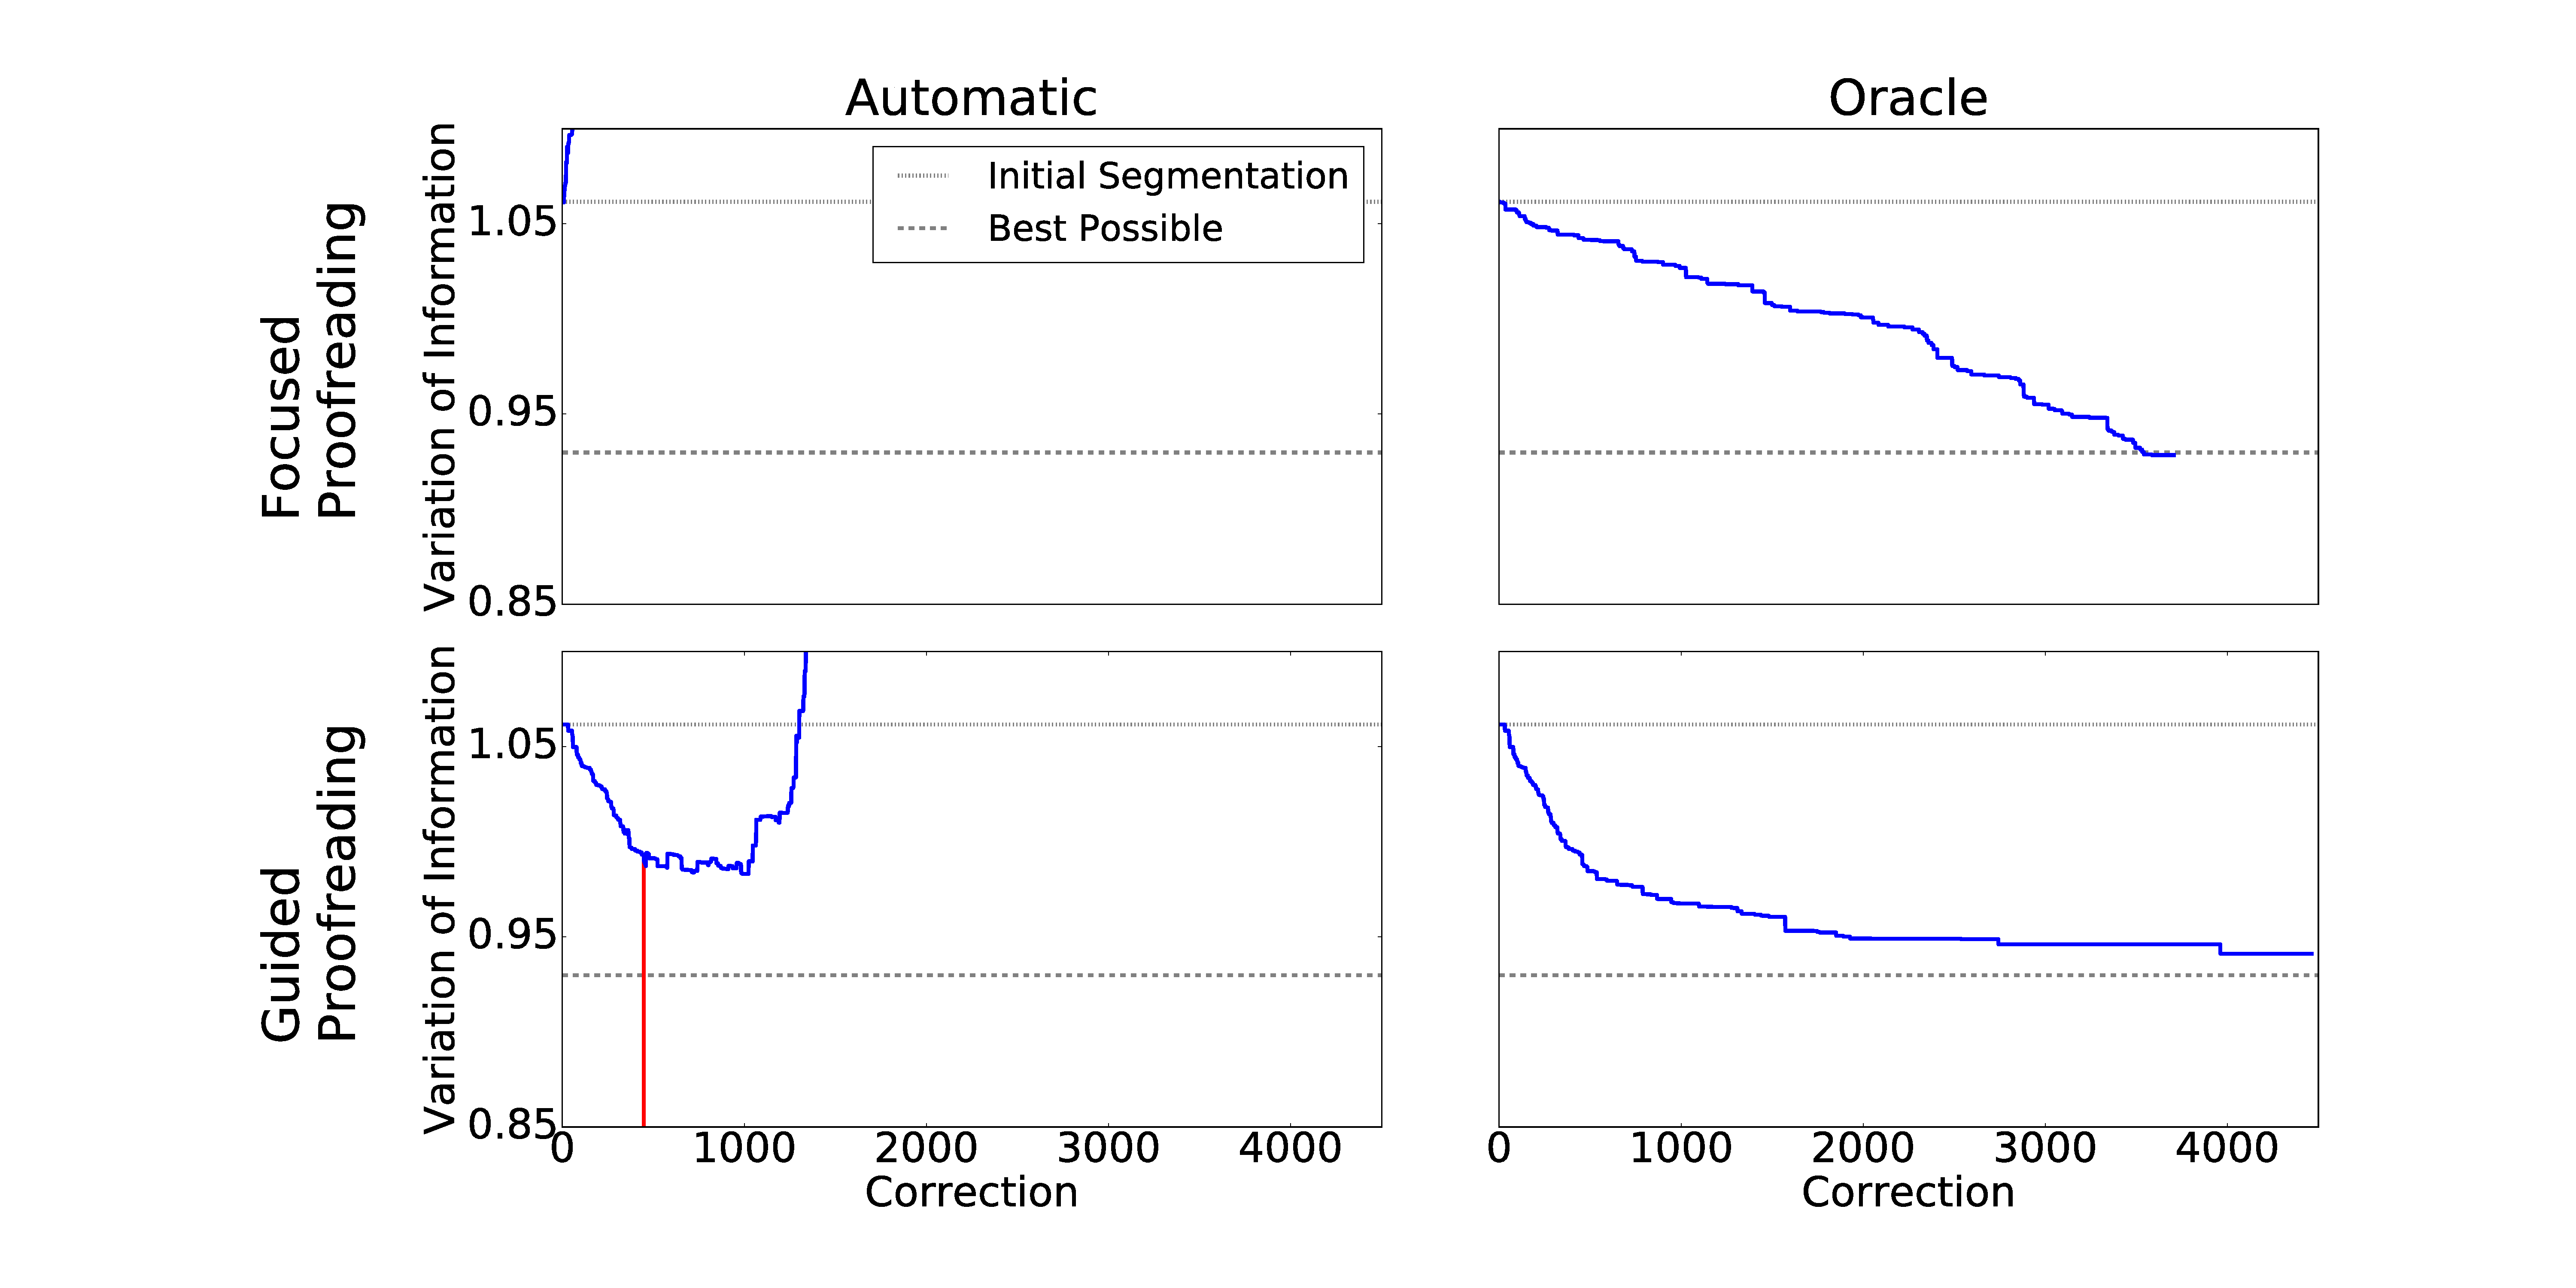
\includegraphics[width=\linewidth]{gfx/cremiAtrails.pdf}
\caption{Performance comparison of Plaza's focused proofreading and our guided proofreading on 5 sections of the CREMI A dataset (split error correction only). All measurements are reported as median VI, the lower the better. The threshold for automatic selection is $p_t=0.95$ (red line). The slope of the selection oracle shows that guided proofreading reduces VI faster.}
\label{fig:cremiAtrails}
\end{figure}

\begin{figure}[t]
\centering
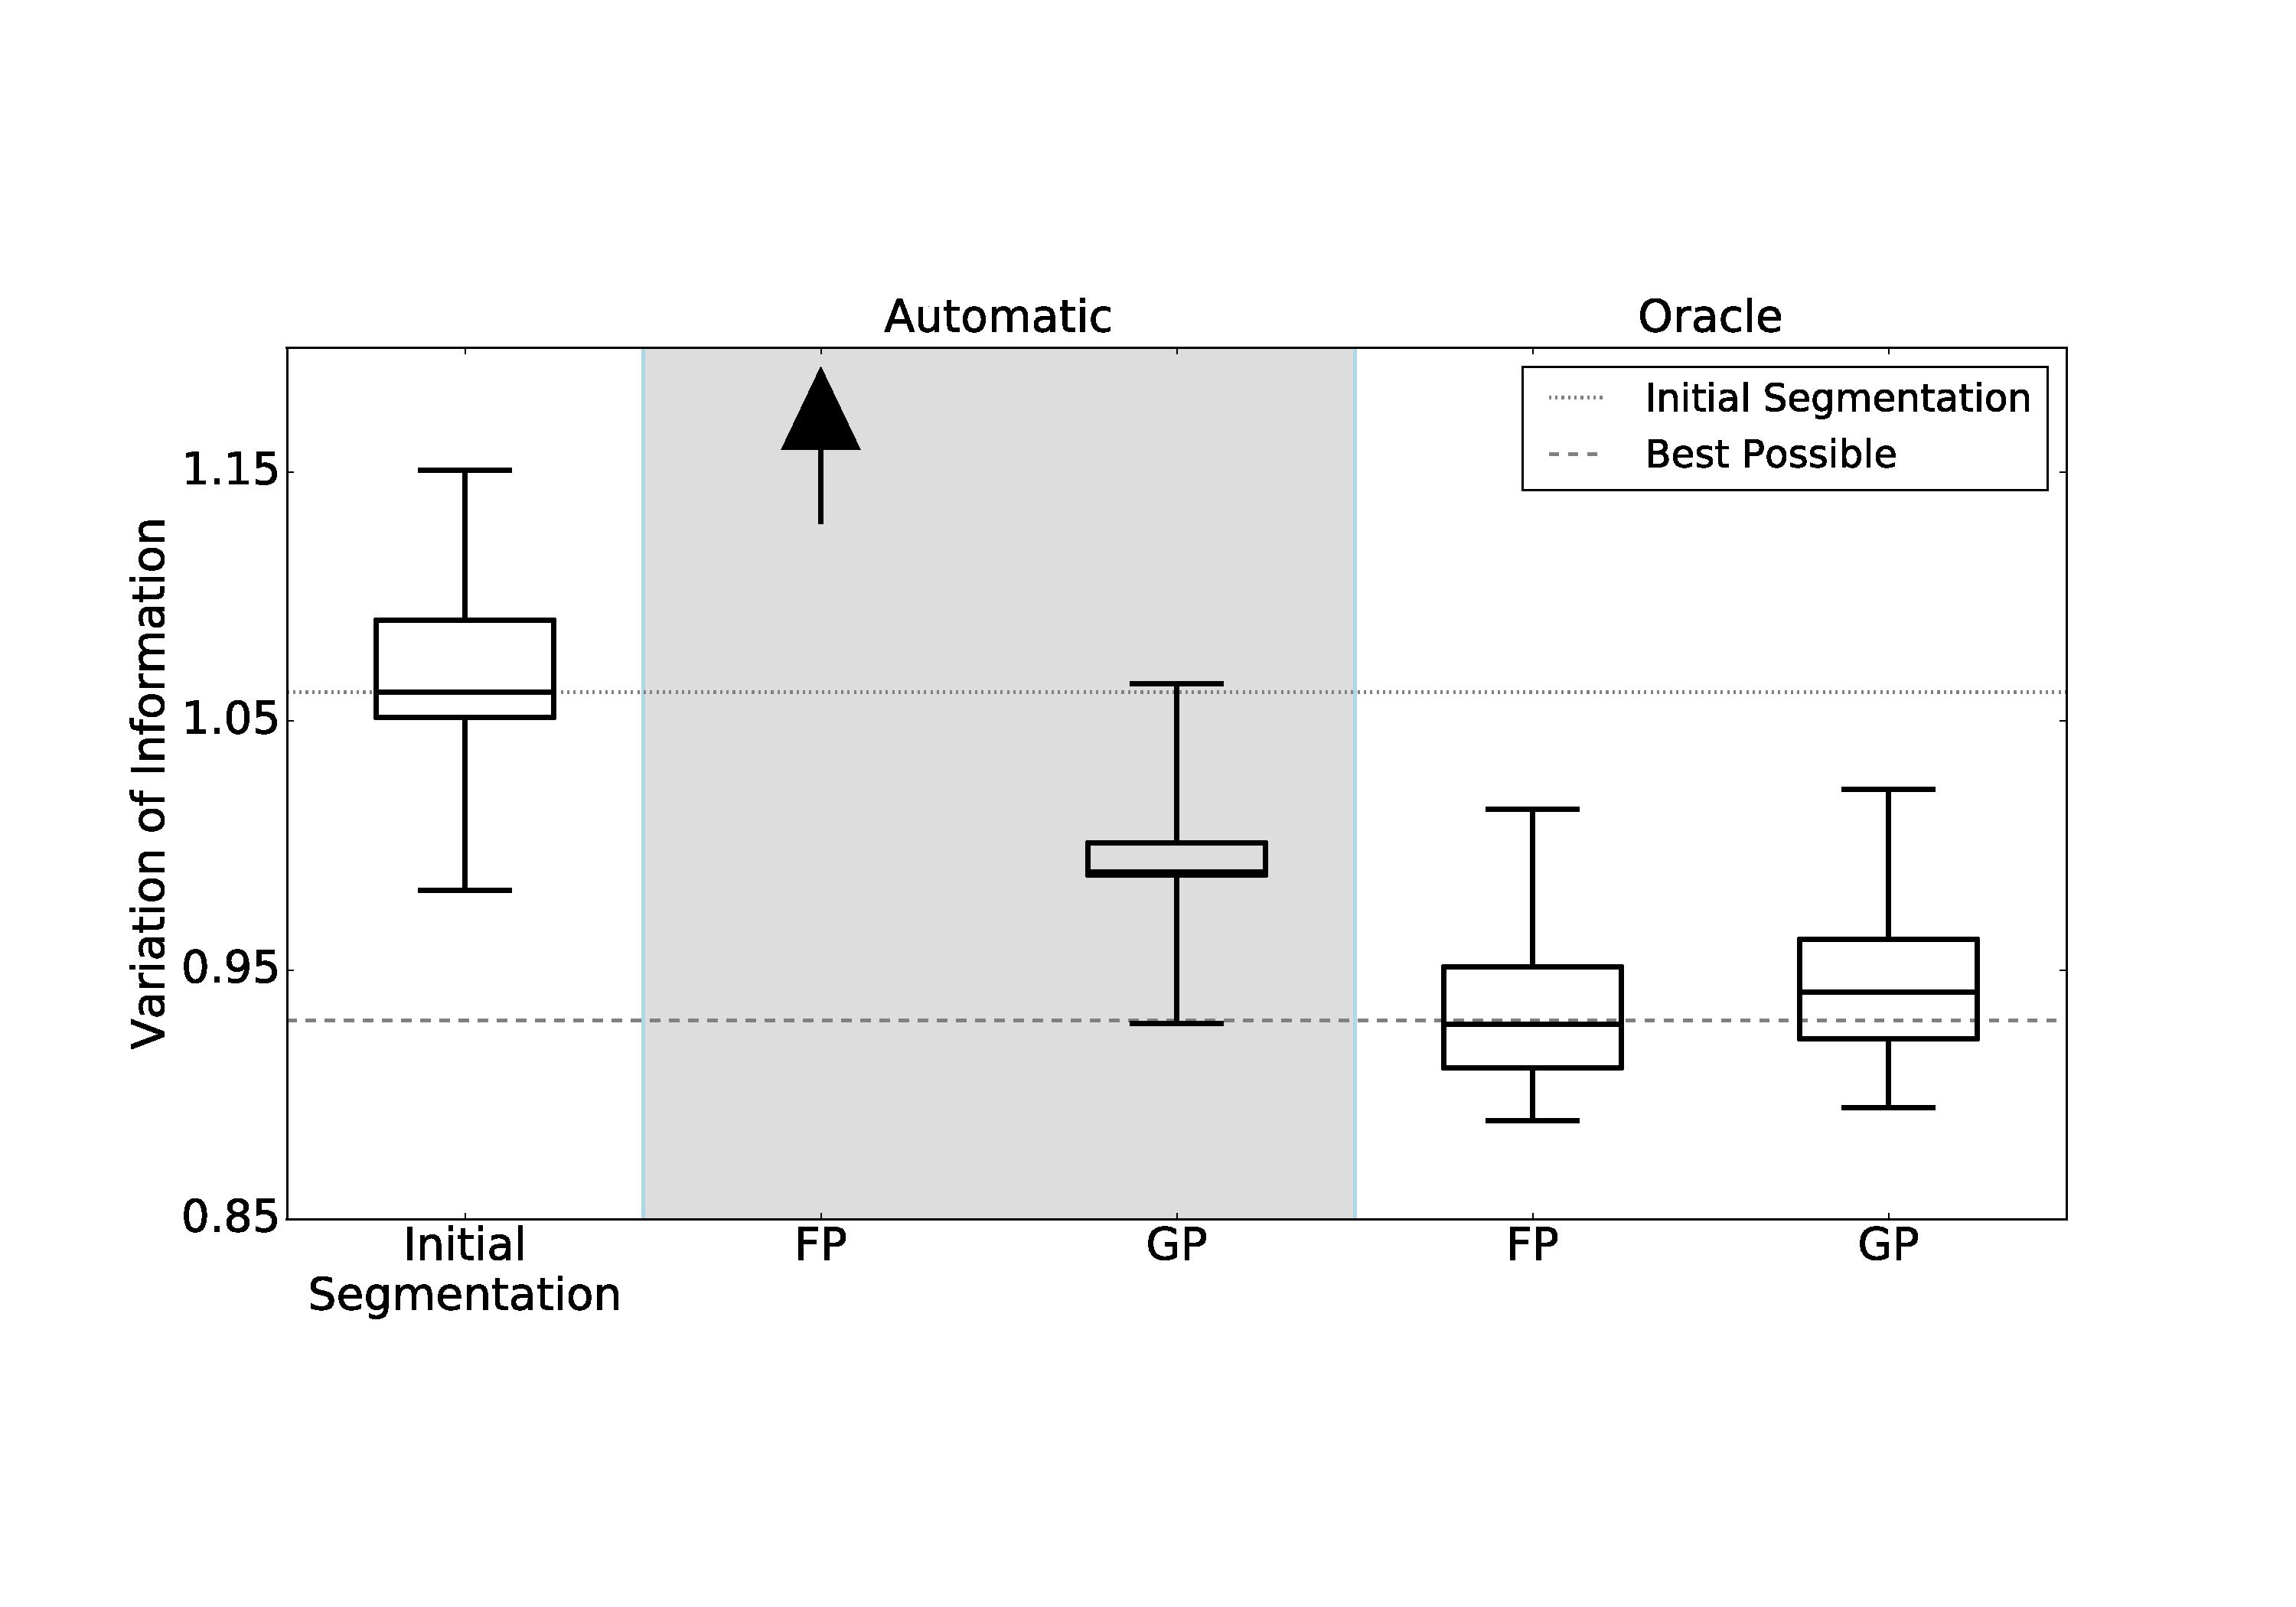
\includegraphics[width=\linewidth]{gfx/cremiAboxplot.pdf}
\caption{VI distributions of guided proofreading (GP) and focused proofreading (FP) output across slices of the CREMI A dataset, with different error correction approaches. The variation resulting from performance of FP with automatic selection is $5.4\times$ higher than GP (as indicated by the arrow), with median VI of $5.32$ and $SD=0.009$. GP does not reach the best possible VI as discussed in the text.}
\label{fig:cremiAboxplot}
\end{figure}

Figure~\ref{fig:cremiAtrails} and~\ref{fig:cremiAboxplot} compare Plaza's focused proofreading and guided proofreading on the 5 sections of the CREMI A dataset.

\paragraph{Selection oracle.} With focused proofreading, the selection oracle reduces median VI to 0.928, $SD=0.043$ from an initial median VI of 1.06 ($SD=0.055$). 532 corrections out of 3707 were accepted. Guided proofreading does not reach the best possible VI, however, reduces VI faster with less corrections to 0.941 ($SD=0.04$). Out of 4463 corrections, 1275 were accepted.

\paragraph{Automatic selection with threshold.} Not surprisingly, focused proofreading performs poorly when ran automatically (VI of 5.32, $SD=0.009$). Guided proofreading is able to reduce VI to 0.989 ($SD=0.043$) with $p_t=0.95$.

\subsection{CREMI B}

Figure~\ref{fig:cremiBtrails} and~\ref{fig:cremiBboxplot} show the results on the CREMI B dataset.

\paragraph{Selection oracle.} Focused proofreading is able to reduce median VI to 1.29, $SD=0.031$ from an initial median VI of 1.63 ($SD=0.025$). Out of 1959 corrections, the selection oracle accepted 517. With guided proofreading, the median VI is reduced to 1.30, $SD=0.03$ while accepting 1111 corrections out of 3073.

\paragraph{Automatic selection with threshold.} Focused proofreading results in a VI of 4.25 ($SD=0.07$). Guided proofreading reduces median VI to 1.43 ($SD=0.038$).

\begin{figure}[t]
\centering
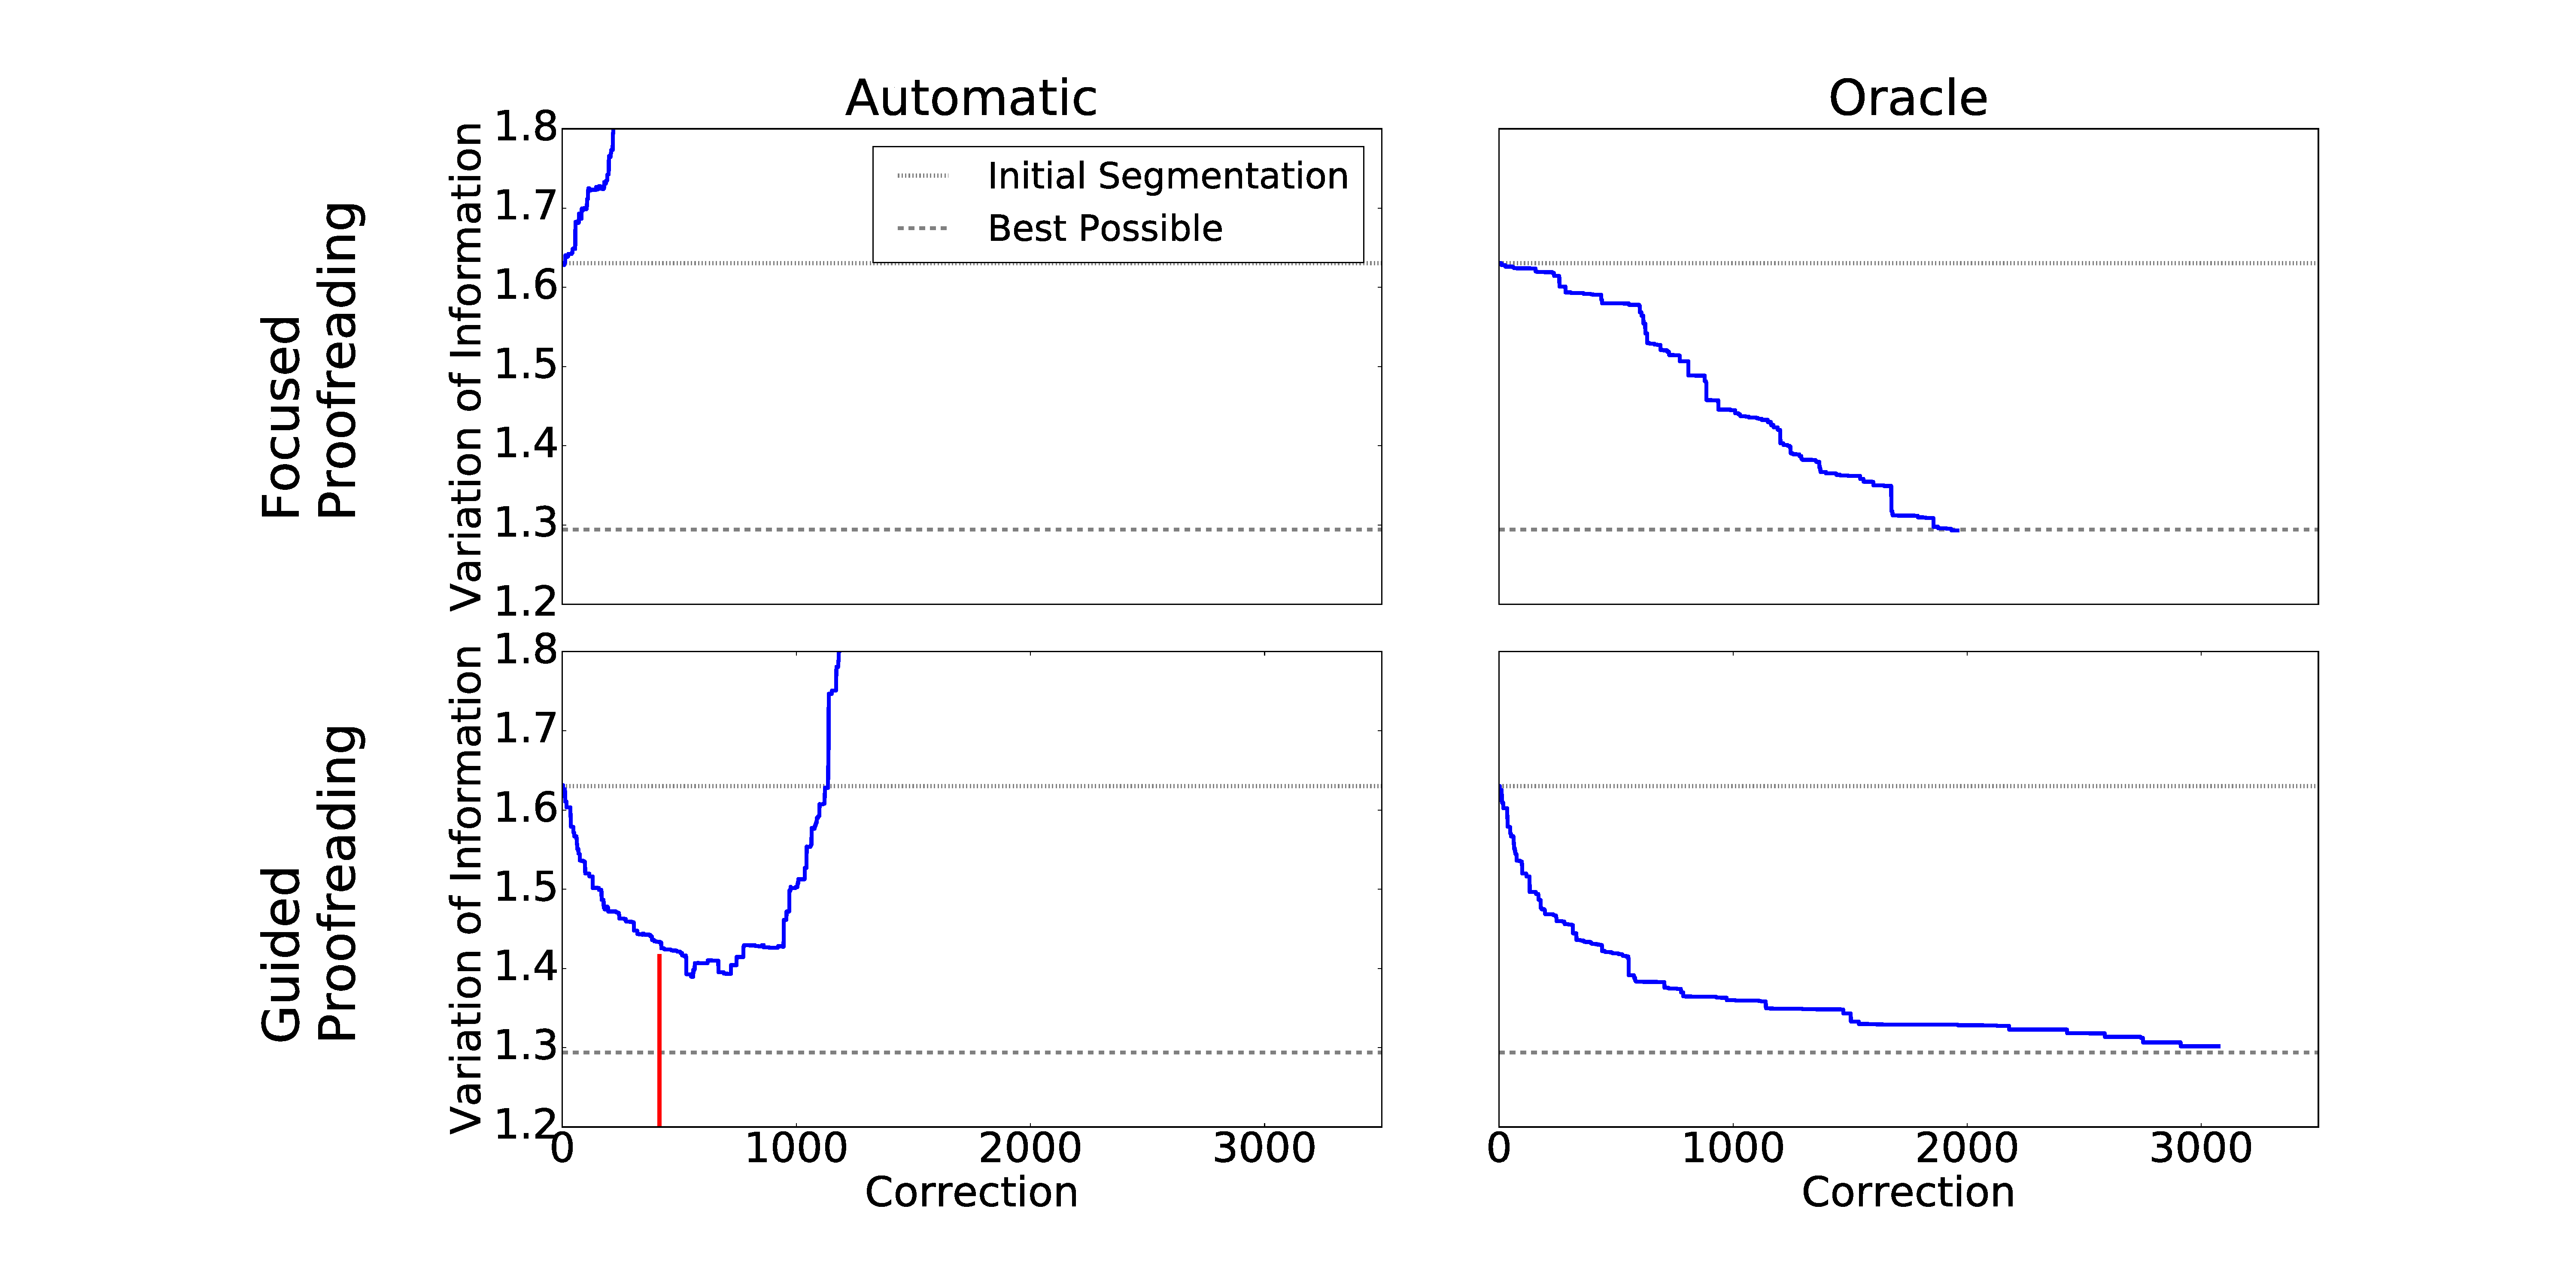
\includegraphics[width=\linewidth]{gfx/cremiBtrails.pdf}
\caption{Split error correction by Plaza's focused proofreading and our guided proofreading compared on the CREMI B dataset. All measurements are reported as median VI, the lower the better. Automatic selection with threshold (red line) yields reasonable performance using guided proofreading.}
\label{fig:cremiBtrails}
\end{figure}

\begin{figure}[t]
\centering
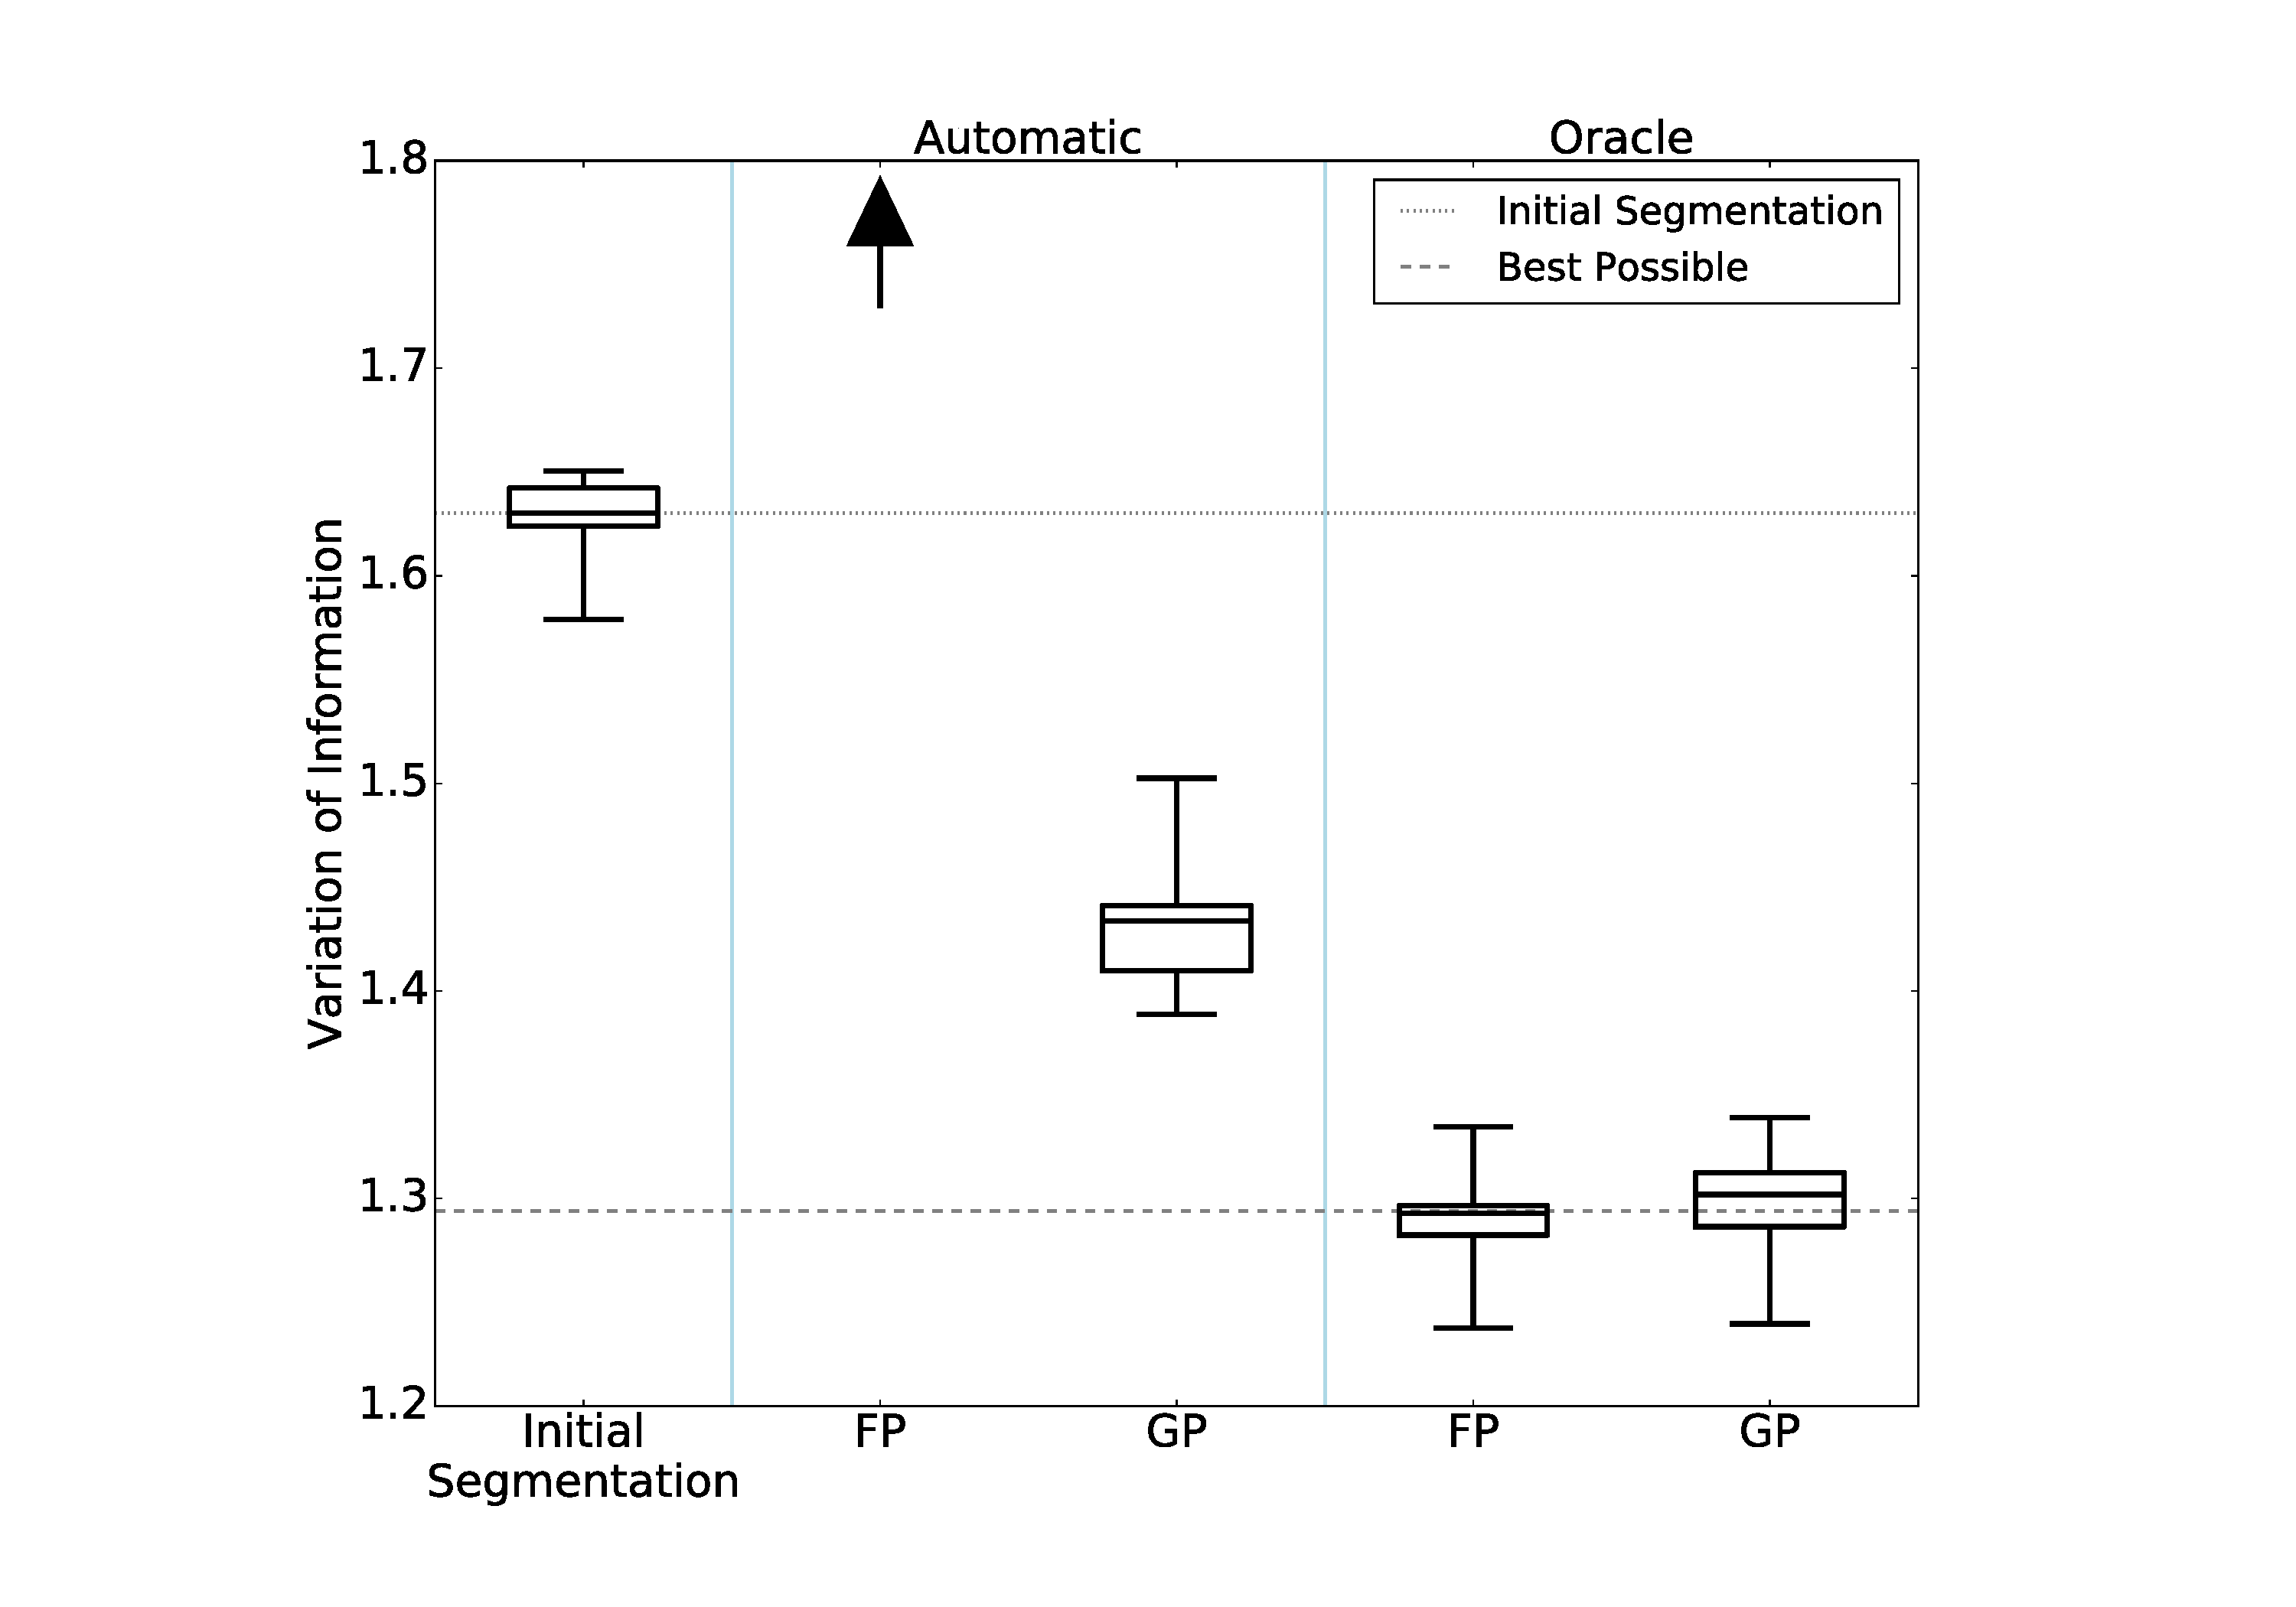
\includegraphics[width=\linewidth]{gfx/cremiBboxplot.pdf}
\caption{VI distributions of guided proofreading (GP) and focused proofreading (FP) output across 5 sections of the CREMI B dataset. We compare automatic selection and oracle selection. The variation resulting from performance of FP with automatic selection is $3\times$ higher than GP (as indicated by the arrow), with median VI of $4.25$ and $SD=0.07$.}
\label{fig:cremiBboxplot}
\end{figure}

\subsection{CREMI C}

The results of split error correction using focused proofreading and guided proofreading on the CREMI C subvolume are shown in Figure~\ref{fig:cremiCtrails} and~\ref{fig:cremiCboxplot}.

\paragraph{Selection oracle.} With focused proofreading, the initial median VI of 1.75 ($SD=0.086$) is reduced to 1.45 ($SD=0.056$) with 670 accepted corrections out of 2694. Guided proofreading is able to reduce the VI to 1.47 ($SD=0.06$). Here, the oracle accepted 1531 out of 4332 corrections. 

\paragraph{Automatic selection with threshold.} Focused proofreading results in a VI of 4.81 ($SD=0.03$). Guided proofreading with $p_t=0.95$ reduces median VI to 1.57 ($SD=0.081$).

\begin{figure}[t]
\centering
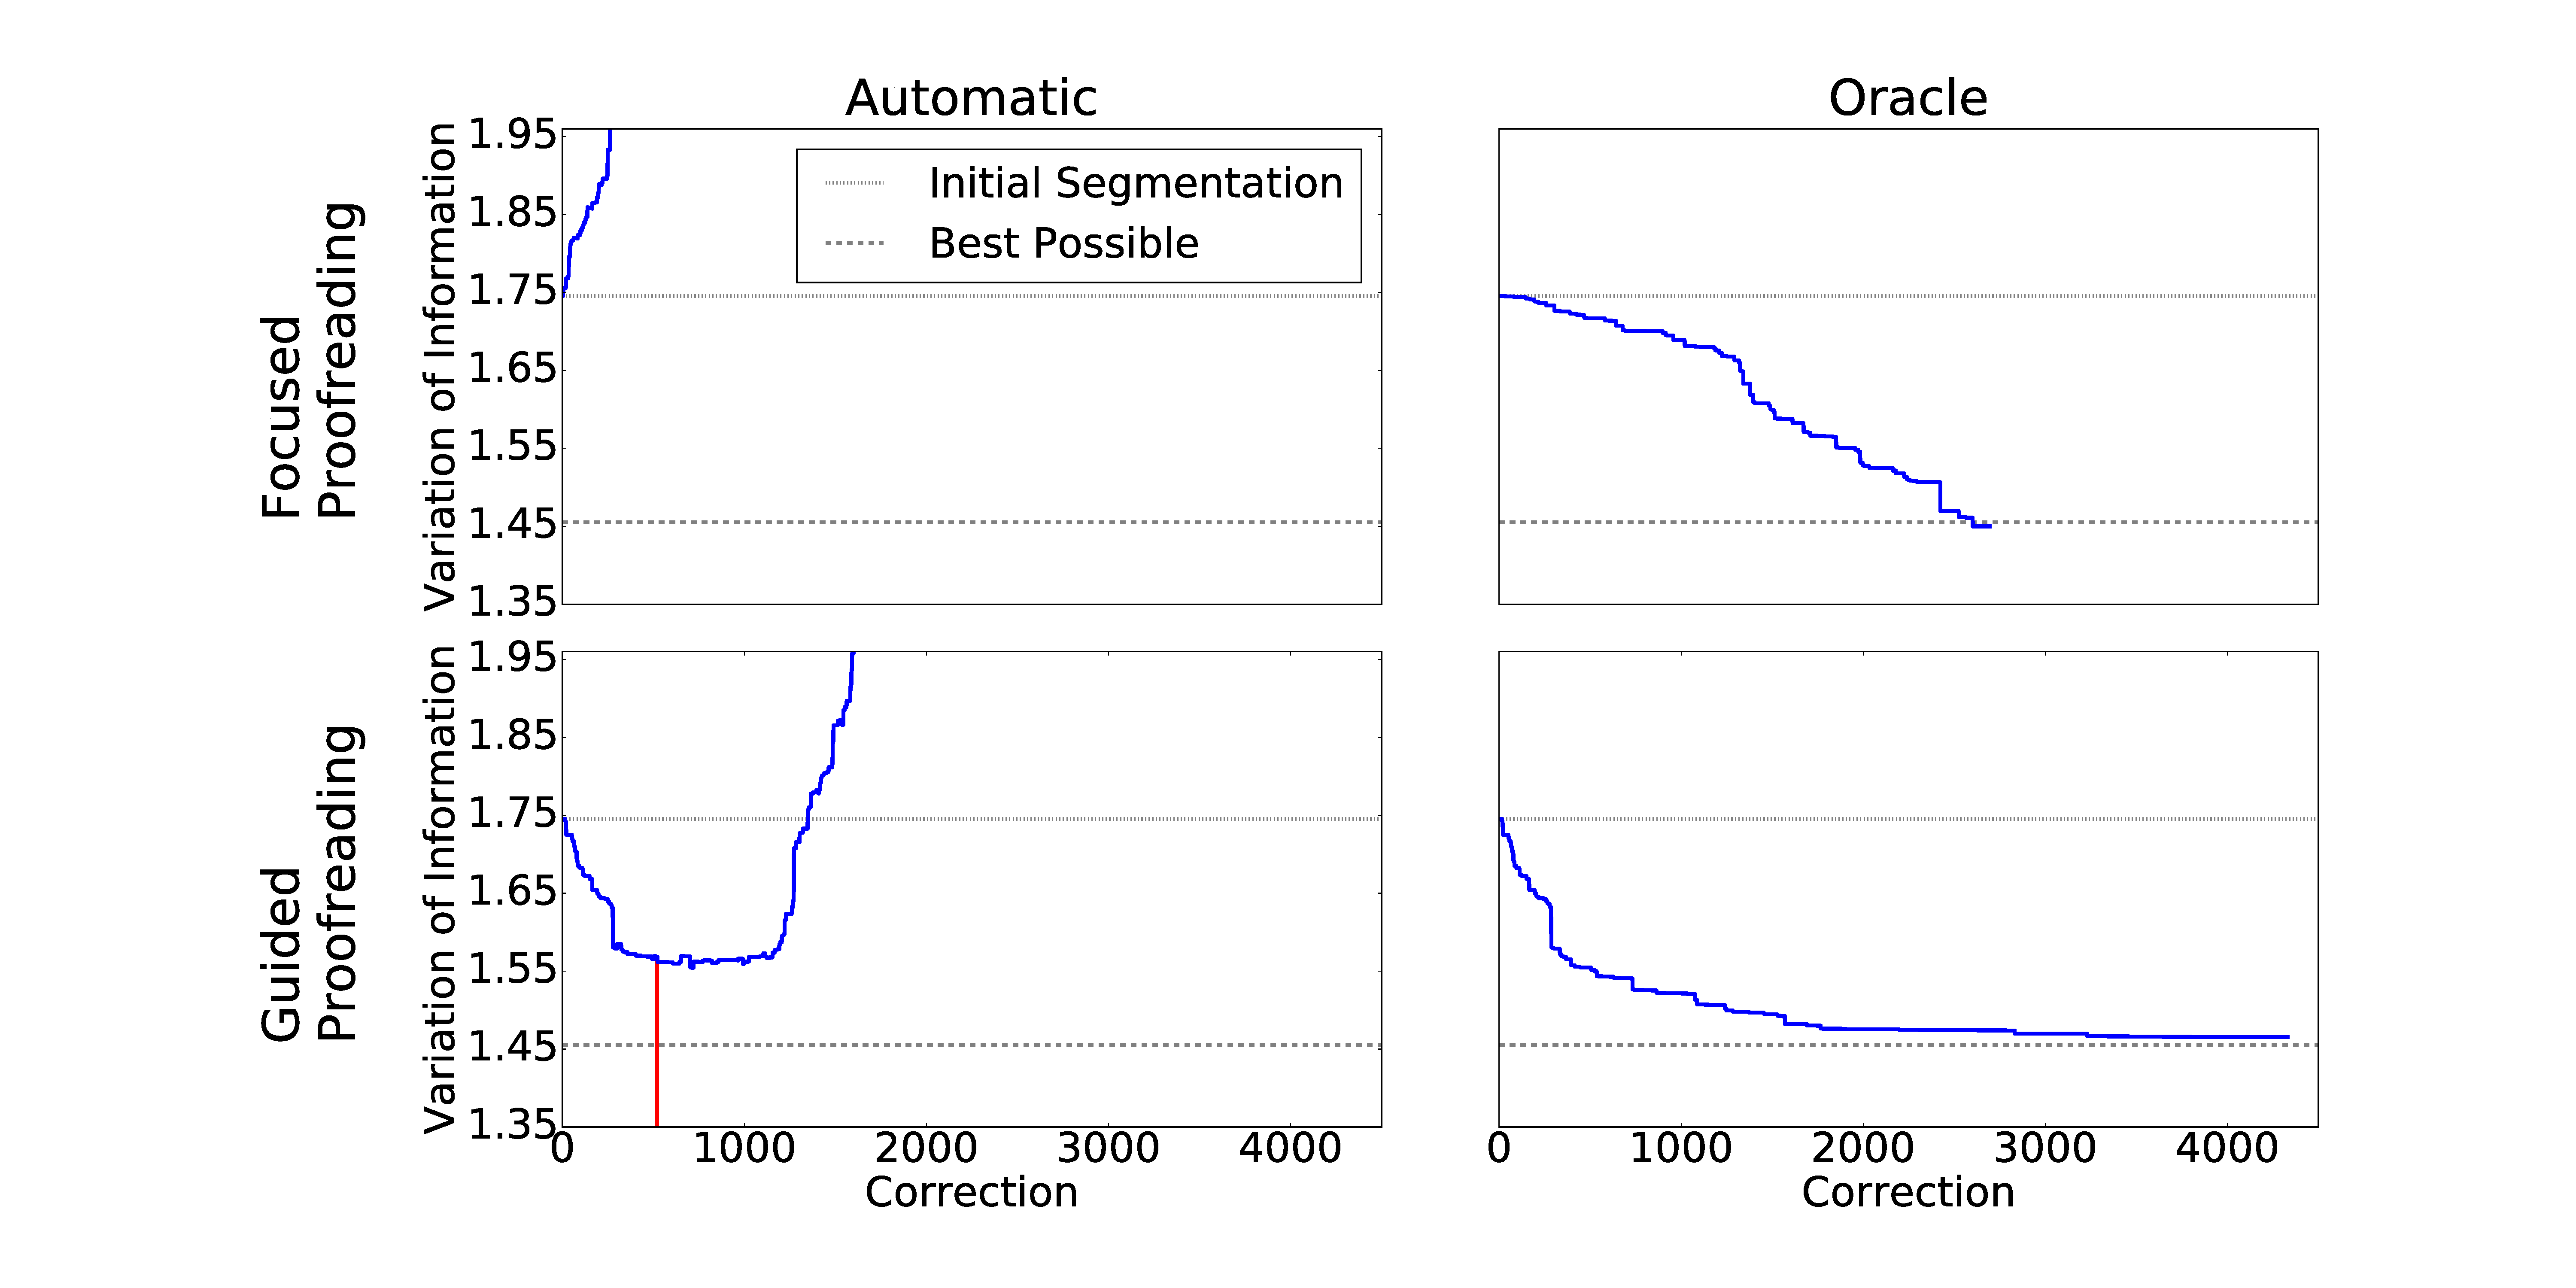
\includegraphics[width=\linewidth]{gfx/cremiCtrails.pdf}
\caption{Performance comparison of Plaza's focused proofreading and our guided proofreading on the CREMI C dataset (only split error correction). Lower VI scores are better. Guided proofreading corrects the initial segmentation faster with less corrections than focused proofreading.}
\label{fig:cremiCtrails}
\end{figure}

\begin{figure}[t]
\centering
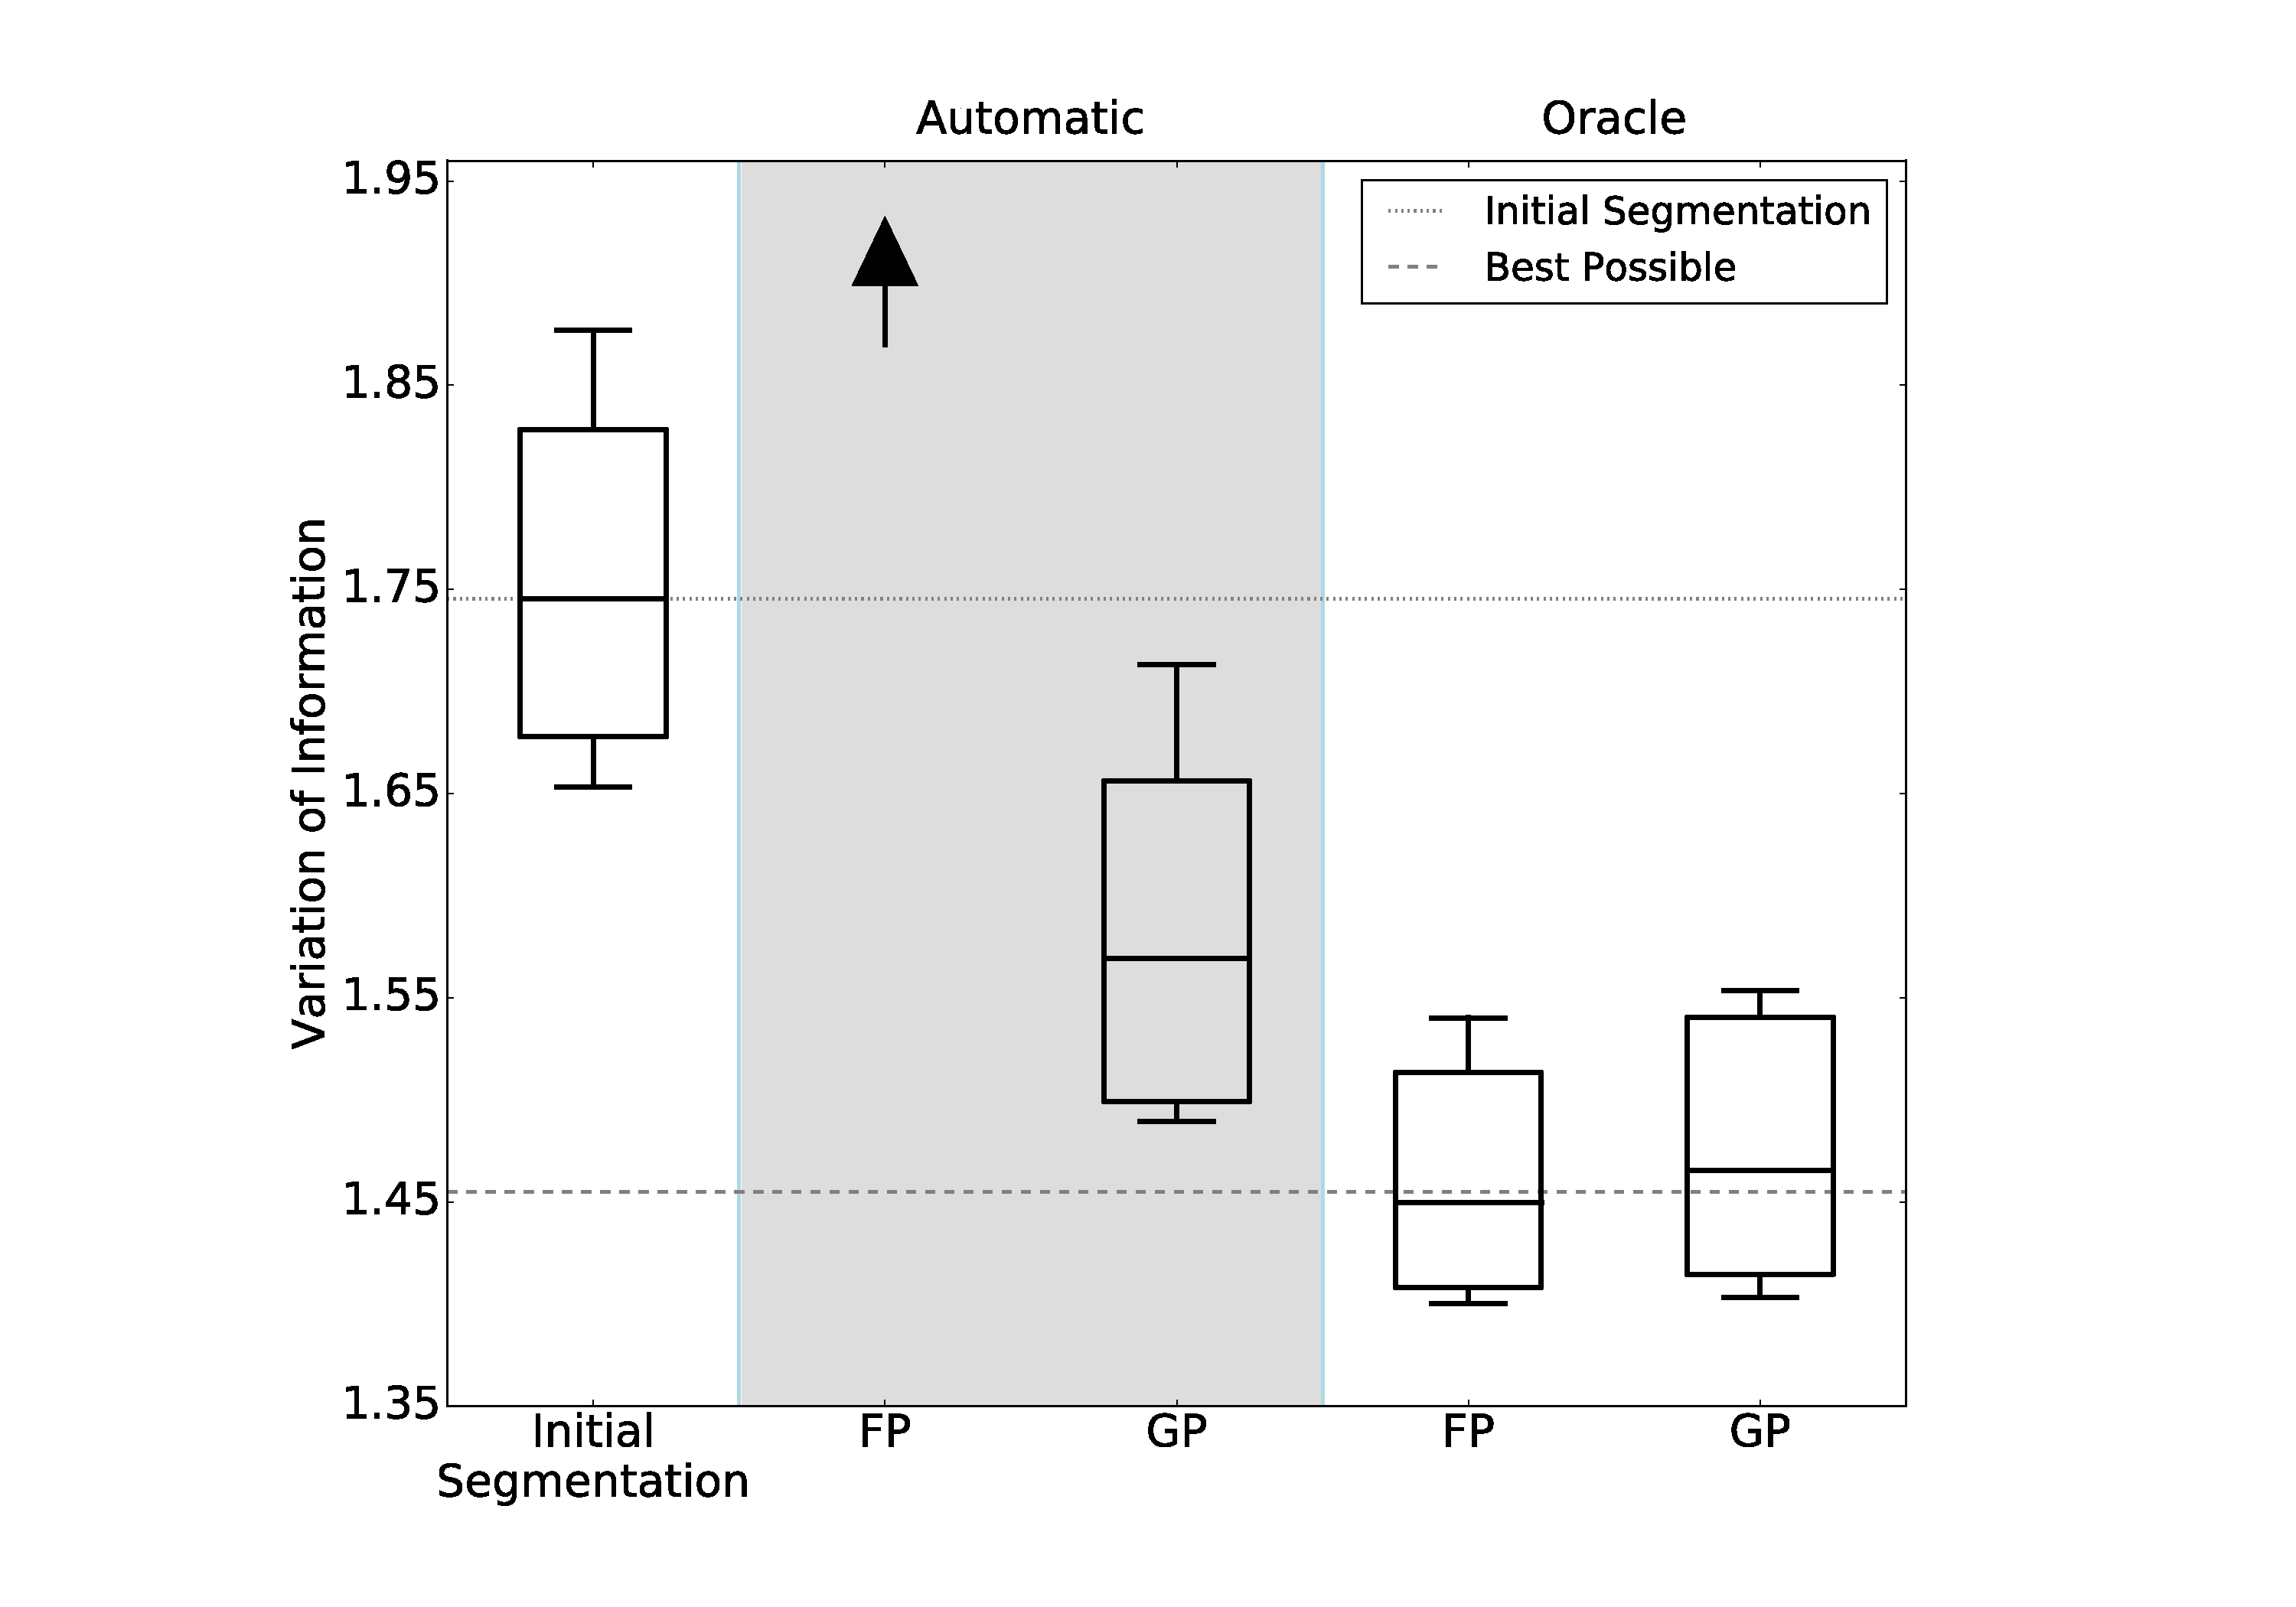
\includegraphics[width=\linewidth]{gfx/cremiCboxplot.pdf}
\caption{VI distributions of guided proofreading (GP) and focused proofreading (FP) output across the CREMI C subvolume, with different error correction approaches. The variation resulting from performance of FP with automatic selection is $3\times$ higher than GP (as indicated by the arrow), with median VI of $4.81$ and $SD=0.08$.}
\label{fig:cremiCboxplot}
\end{figure}


\section{Forced Choice User Experiment}

\subsection{Recruitment and Participation}

Novice participants were recruited via flyer (figure~\ref{fig:flyer}). An anonymized listing of all participants including demographic information is shown in table~\ref{tab:participants}.

\begin{figure}[t]
\centering

\includegraphics[width=\linewidth]{gfx/flyer_anon.pdf}
\caption{Participants were recruited with this flyer.}
\label{fig:flyer}
\end{figure}

\begin{figure}[t]
\centering
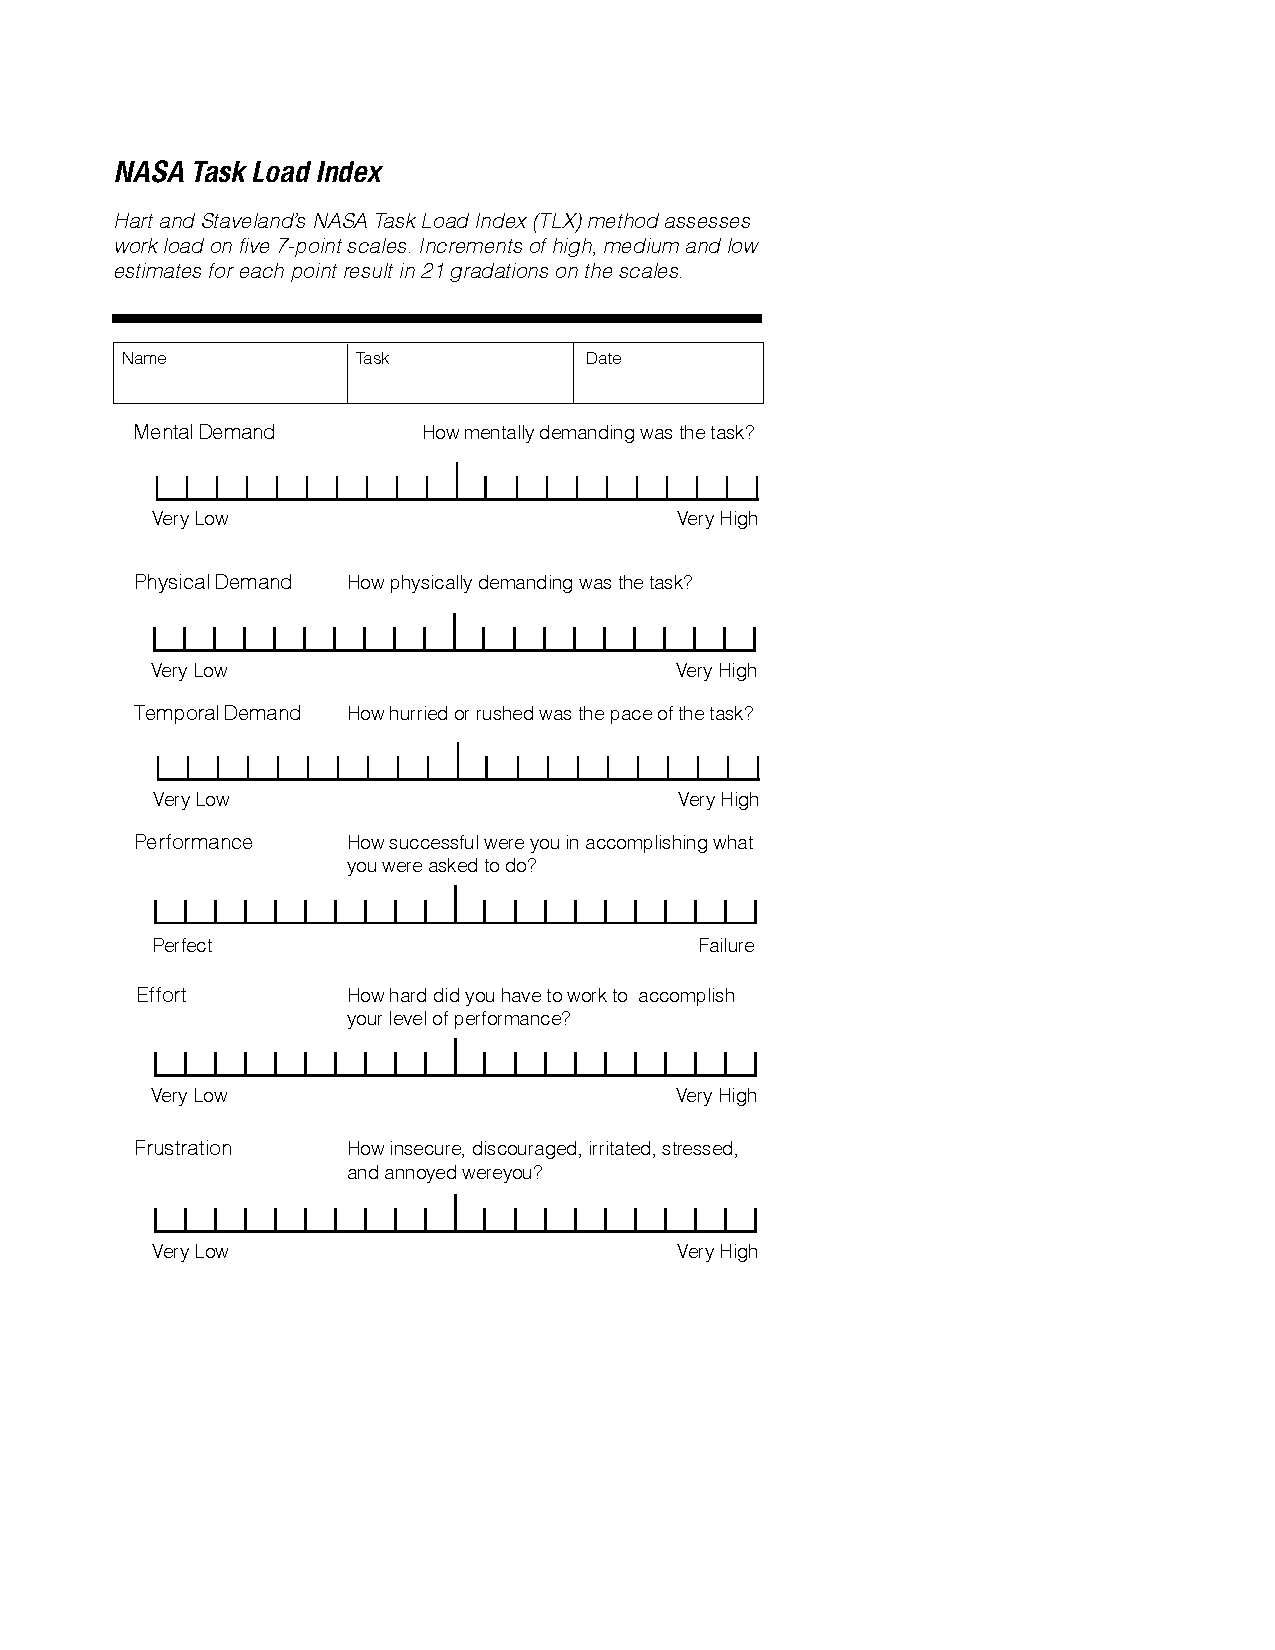
\includegraphics[width=\linewidth]{gfx/NASA_TXL.pdf}
\caption{The NASA-TLX workload index to record subjective responses.}
\label{fig:nasatxl}
\end{figure}


\begin{table}[t]
\caption{The novice participants ($N=20$) of the forced choice user experiment. The table shows sex (20 female), age ($M=30$) and the randomly assigned classifier (focused proofreading as FP, guided proofreading as GP).}%While the training of our classifier is more expensive, testing accuracy is superior. }

\small{
\begin{tabular}{@{}l|c|c|c@{}}
	\toprule
     \textbf{ID} & \textbf{Sex} &  \textbf{Age} & \textbf{Classifier}  \\ \midrule	
S38 &		F & 20 & FP \\
S57&		F & 30 & FP \\ 
S32&		M & 38 & FP \\
S34&		F & 21 & FP \\
S21&		F & 65 & FP \\
S9 &	M & 33 & FP \\
S45 &		M & 28 & FP \\
S31&		M & 27 & FP \\
S24&		F & 21 & FP \\
S6	&	F & 38 & FP \\
S28	&	M&	32& GP \\
S36	&	F&	19& GP \\
S35	&	M&	26& GP \\
S25	&	M&	26& GP \\
S54	&	F&	30& GP \\
S53	&	M&	29& GP \\
S52	&	M	&27& GP \\
S51&		M&	31& GP \\
S200	 &	F	&37& GP \\
S3	 &F&	30 & GP



\end{tabular}
\hspace{2mm}
}
\label{tab:participants}
\end{table}

\subsection{User Interface}

\CHANGED{We integrate guided proofreading into an existing large data connectomics workflow. The web-based system is designed with a novice-friendly user interface (Fig. 5 in the paper, and the supplemental video). We show the current labeling of a cell boundary outline and its proposed correction overlayed on EM image data. The user cannot distinguish the current labeling from the proposed correction to avoid selection bias. We also show a solid overlay of the current and the proposed labeling. In addition, we show the image without overlays to provide an unoccluded view. User interaction is simple and involves one mouse click on either the current labeling or the correction. After interaction, the next potential error is shown.}

\subsection{Example Classifications}

During the user study, participants were asked to accept or reject potential errors and their corrections --- some more difficult than others. Figure~\ref{fig:patches} shows a selection of potential errors and their corrections.

\begin{figure}[t]
\centering
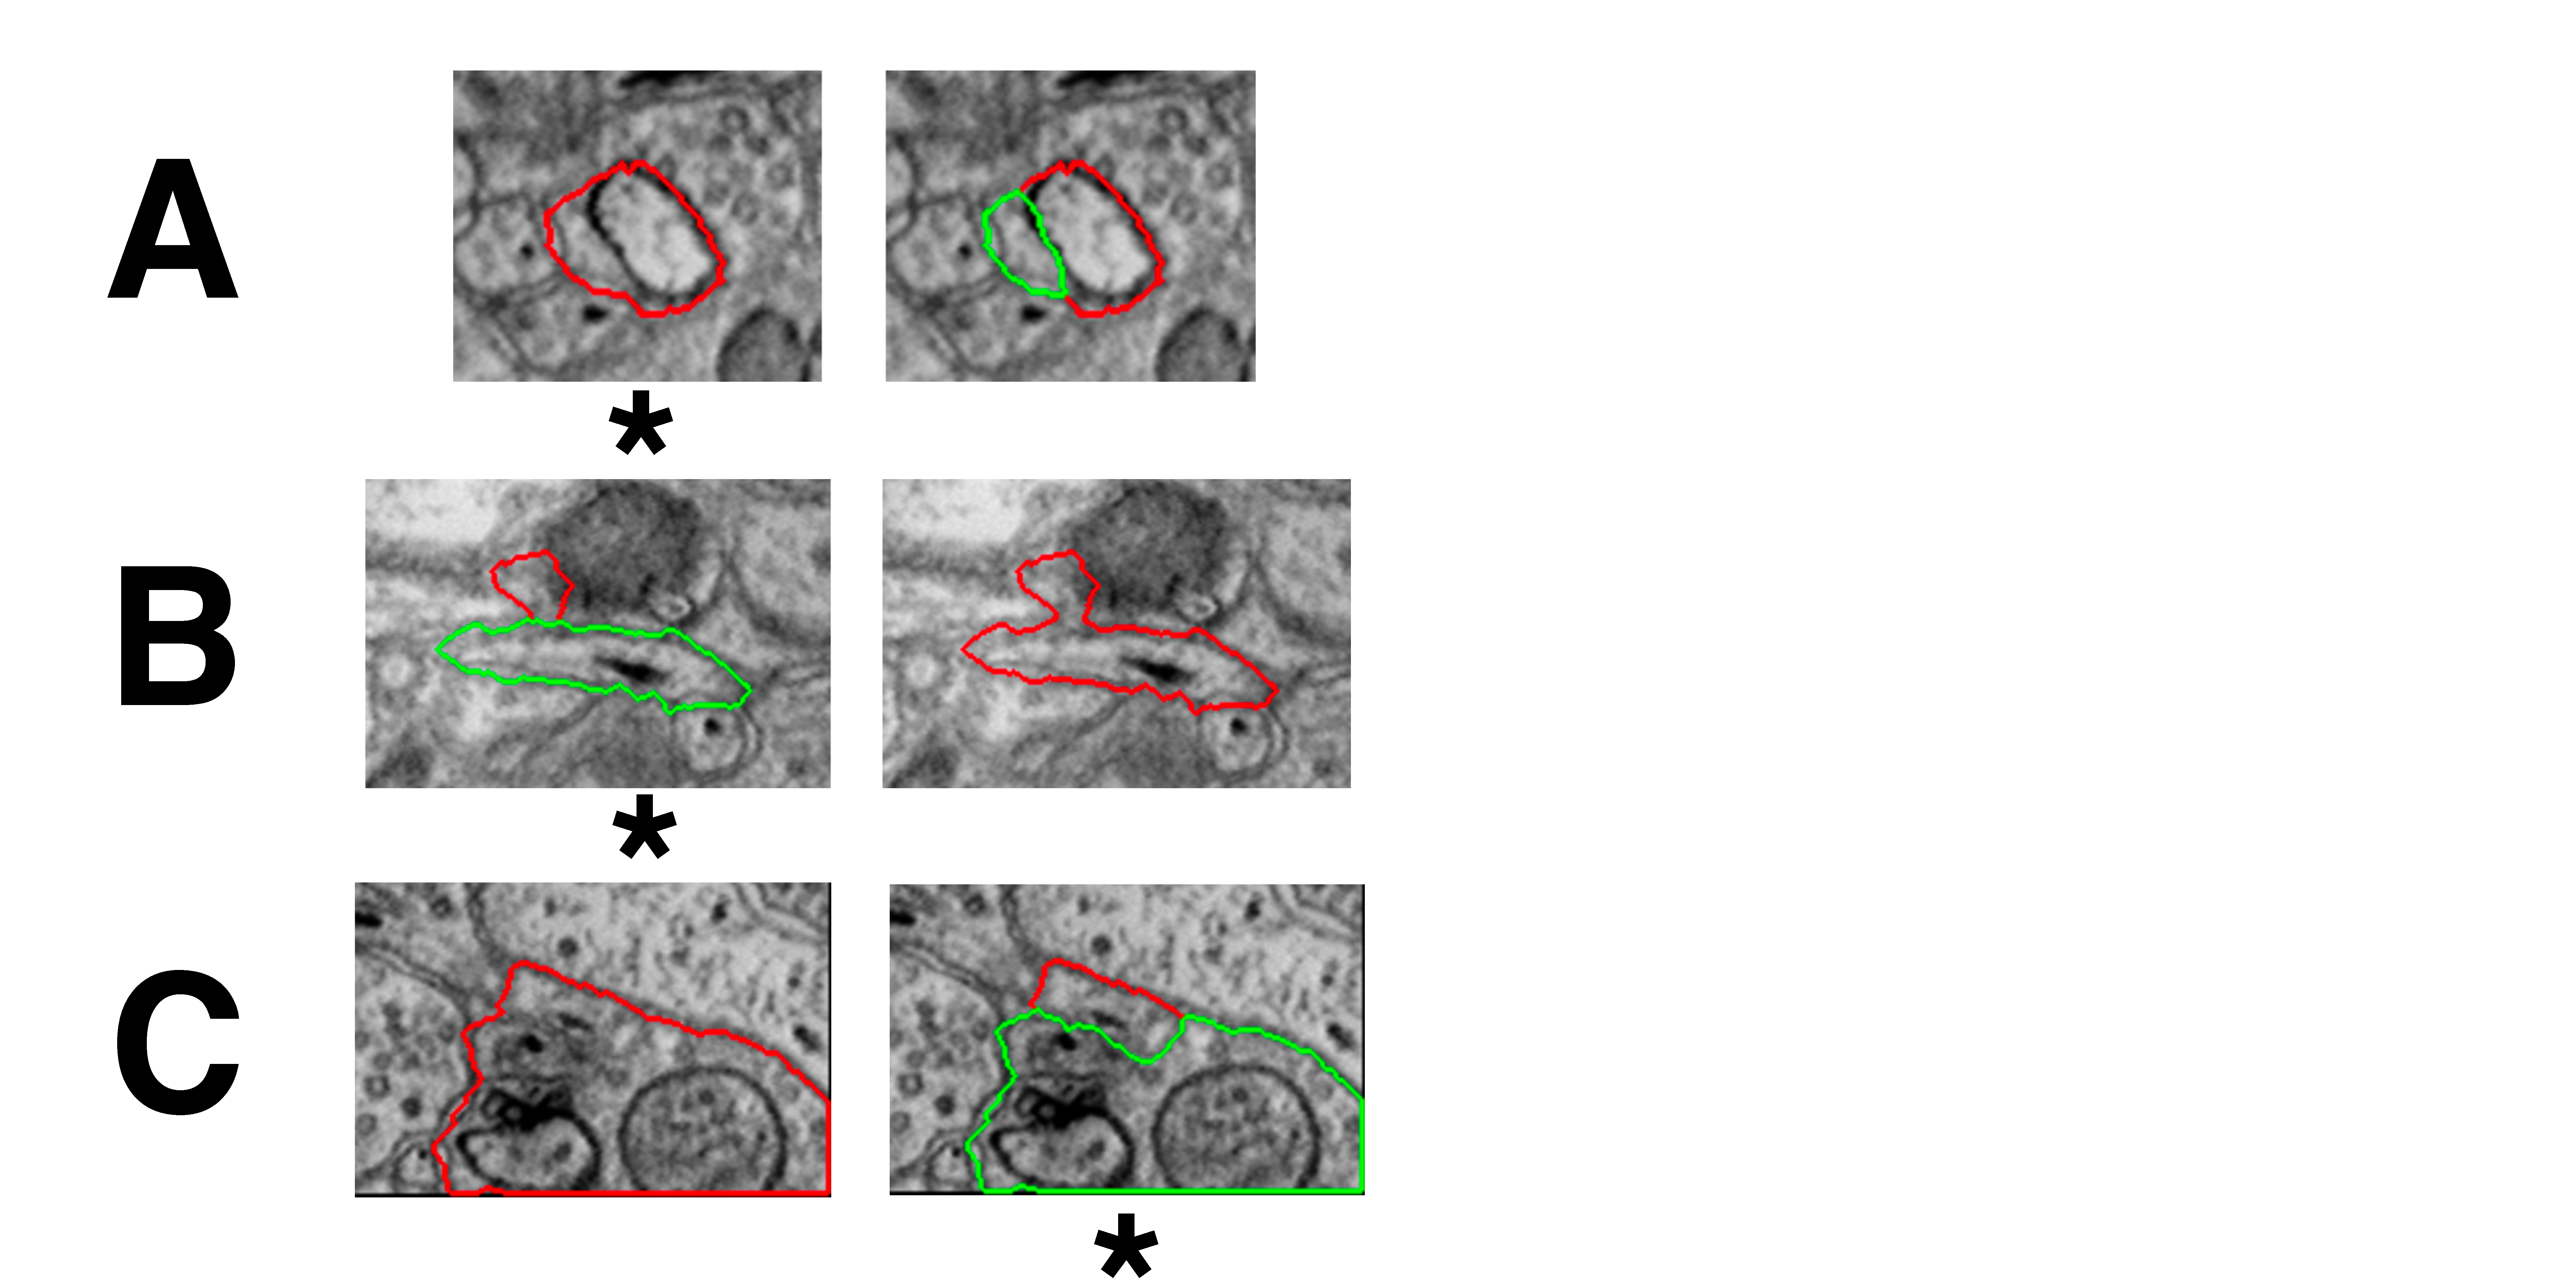
\includegraphics[width=\linewidth]{gfx/patches.pdf}
\caption{A selection of suggested errors and potential corrections during the forced choice user experiment. The star (*) indicates which choice reduces VI. While all participants were able to correctly choose for patch A, only few were able to correctly choose for patch B and C.}
\label{fig:patches}
\end{figure}

\subsection{Subjective Responses}

After the experiment, we acquired subjective responses using the NASA-TLX task load index (Figure~\ref{fig:nasatxl}). We performed ANOVA to test for statistical significance~\cite{shaffer1995}. Mental, physical, and temporal demands were reported slightly higher for participants using focused proofreading but the analysis did not yield any significance. \CHANGED{This is unsurprising as the user interface was the same for both groups.}

\begin{itemize}
\item \textbf{Mental Demand.} Participants using focused proofreading stated a higher mental demand $M=11.5$ ($SD=2.098$) than with guided proofreading $M=8.1$ ($SD=2.003$). This was not statistically significant ($F_{1,18}=3.2574, p=0.3695$).
\item \textbf{Physical Demand.} While naturally physical demand was rated low, participants using focused proofreading stated it slightly higher $M=5.4$ ($SD=2.26$) than with guided proofreading $M=2.9$ ($SD=1.76$). This was not statistically significant ($F_{1,18}=1.7507, p=0.5454$).
\item \textbf{Temporal Demand.} For temporal demand, participants using focused proofreading $M=8.4$ ($SD=1.95$) reported almost equal to guided proofreading $M=8.3$ ($SD=1.99$). This was not statistically significant ($F_{1,18}=0.0033, p=0.9987$).
\item \textbf{Performance.} Here, participants were asked to rate their own performance. All participants rated their performance as pretty well (the lower, the better). For focused proofreading $M=6.8$ ($SD=1.97$) and for guided proofreading $M=7.8$ ($SD=2.04$). This was not statistically significant ($F_{1,18}=0.3091, p=0.8878$).
\item \textbf{Effort.} Participants using focused proofreading stated higher effort $M=13.0$ ($SD=2.336$) than with guided proofreading $M=10.6$ ($SD=2.127$). This was not statistically significant ($F_{1,18}=1.1459, p=0.6599$).
\item \textbf{Frustration.} Participants overall reported low frustration. Reported were $M=5.0$ ($SD=1.90$) using focused proofreading and $M=5.9$ ($SD=185$) using guided proofreading. This was not statistically significant ($F_{1,18}=0.3271, p=0.8818$).
\end{itemize}

{\small
\bibliographystyle{ieee}
\bibliography{connectomics}
}

\end{document}
